\documentclass[]{article}
\usepackage{lmodern}
\usepackage{amssymb,amsmath}
\usepackage{ifxetex,ifluatex}
\usepackage{fixltx2e} % provides \textsubscript
\ifnum 0\ifxetex 1\fi\ifluatex 1\fi=0 % if pdftex
  \usepackage[T1]{fontenc}
  \usepackage[utf8]{inputenc}
\else % if luatex or xelatex
  \ifxetex
    \usepackage{mathspec}
  \else
    \usepackage{fontspec}
  \fi
  \defaultfontfeatures{Ligatures=TeX,Scale=MatchLowercase}
\fi
% use upquote if available, for straight quotes in verbatim environments
\IfFileExists{upquote.sty}{\usepackage{upquote}}{}
% use microtype if available
\IfFileExists{microtype.sty}{%
\usepackage{microtype}
\UseMicrotypeSet[protrusion]{basicmath} % disable protrusion for tt fonts
}{}
\usepackage[margin=1in]{geometry}
\usepackage{hyperref}
\hypersetup{unicode=true,
            pdftitle={12 Practical likelihood-based inference for POMP models},
            pdfauthor={Edward Ionides},
            pdfborder={0 0 0},
            breaklinks=true}
\urlstyle{same}  % don't use monospace font for urls
\usepackage{color}
\usepackage{fancyvrb}
\newcommand{\VerbBar}{|}
\newcommand{\VERB}{\Verb[commandchars=\\\{\}]}
\DefineVerbatimEnvironment{Highlighting}{Verbatim}{commandchars=\\\{\}}
% Add ',fontsize=\small' for more characters per line
\usepackage{framed}
\definecolor{shadecolor}{RGB}{248,248,248}
\newenvironment{Shaded}{\begin{snugshade}}{\end{snugshade}}
\newcommand{\KeywordTok}[1]{\textcolor[rgb]{0.13,0.29,0.53}{\textbf{#1}}}
\newcommand{\DataTypeTok}[1]{\textcolor[rgb]{0.13,0.29,0.53}{#1}}
\newcommand{\DecValTok}[1]{\textcolor[rgb]{0.00,0.00,0.81}{#1}}
\newcommand{\BaseNTok}[1]{\textcolor[rgb]{0.00,0.00,0.81}{#1}}
\newcommand{\FloatTok}[1]{\textcolor[rgb]{0.00,0.00,0.81}{#1}}
\newcommand{\ConstantTok}[1]{\textcolor[rgb]{0.00,0.00,0.00}{#1}}
\newcommand{\CharTok}[1]{\textcolor[rgb]{0.31,0.60,0.02}{#1}}
\newcommand{\SpecialCharTok}[1]{\textcolor[rgb]{0.00,0.00,0.00}{#1}}
\newcommand{\StringTok}[1]{\textcolor[rgb]{0.31,0.60,0.02}{#1}}
\newcommand{\VerbatimStringTok}[1]{\textcolor[rgb]{0.31,0.60,0.02}{#1}}
\newcommand{\SpecialStringTok}[1]{\textcolor[rgb]{0.31,0.60,0.02}{#1}}
\newcommand{\ImportTok}[1]{#1}
\newcommand{\CommentTok}[1]{\textcolor[rgb]{0.56,0.35,0.01}{\textit{#1}}}
\newcommand{\DocumentationTok}[1]{\textcolor[rgb]{0.56,0.35,0.01}{\textbf{\textit{#1}}}}
\newcommand{\AnnotationTok}[1]{\textcolor[rgb]{0.56,0.35,0.01}{\textbf{\textit{#1}}}}
\newcommand{\CommentVarTok}[1]{\textcolor[rgb]{0.56,0.35,0.01}{\textbf{\textit{#1}}}}
\newcommand{\OtherTok}[1]{\textcolor[rgb]{0.56,0.35,0.01}{#1}}
\newcommand{\FunctionTok}[1]{\textcolor[rgb]{0.00,0.00,0.00}{#1}}
\newcommand{\VariableTok}[1]{\textcolor[rgb]{0.00,0.00,0.00}{#1}}
\newcommand{\ControlFlowTok}[1]{\textcolor[rgb]{0.13,0.29,0.53}{\textbf{#1}}}
\newcommand{\OperatorTok}[1]{\textcolor[rgb]{0.81,0.36,0.00}{\textbf{#1}}}
\newcommand{\BuiltInTok}[1]{#1}
\newcommand{\ExtensionTok}[1]{#1}
\newcommand{\PreprocessorTok}[1]{\textcolor[rgb]{0.56,0.35,0.01}{\textit{#1}}}
\newcommand{\AttributeTok}[1]{\textcolor[rgb]{0.77,0.63,0.00}{#1}}
\newcommand{\RegionMarkerTok}[1]{#1}
\newcommand{\InformationTok}[1]{\textcolor[rgb]{0.56,0.35,0.01}{\textbf{\textit{#1}}}}
\newcommand{\WarningTok}[1]{\textcolor[rgb]{0.56,0.35,0.01}{\textbf{\textit{#1}}}}
\newcommand{\AlertTok}[1]{\textcolor[rgb]{0.94,0.16,0.16}{#1}}
\newcommand{\ErrorTok}[1]{\textcolor[rgb]{0.64,0.00,0.00}{\textbf{#1}}}
\newcommand{\NormalTok}[1]{#1}
\usepackage{graphicx,grffile}
\makeatletter
\def\maxwidth{\ifdim\Gin@nat@width>\linewidth\linewidth\else\Gin@nat@width\fi}
\def\maxheight{\ifdim\Gin@nat@height>\textheight\textheight\else\Gin@nat@height\fi}
\makeatother
% Scale images if necessary, so that they will not overflow the page
% margins by default, and it is still possible to overwrite the defaults
% using explicit options in \includegraphics[width, height, ...]{}
\setkeys{Gin}{width=\maxwidth,height=\maxheight,keepaspectratio}
\IfFileExists{parskip.sty}{%
\usepackage{parskip}
}{% else
\setlength{\parindent}{0pt}
\setlength{\parskip}{6pt plus 2pt minus 1pt}
}
\setlength{\emergencystretch}{3em}  % prevent overfull lines
\providecommand{\tightlist}{%
  \setlength{\itemsep}{0pt}\setlength{\parskip}{0pt}}
\setcounter{secnumdepth}{0}
% Redefines (sub)paragraphs to behave more like sections
\ifx\paragraph\undefined\else
\let\oldparagraph\paragraph
\renewcommand{\paragraph}[1]{\oldparagraph{#1}\mbox{}}
\fi
\ifx\subparagraph\undefined\else
\let\oldsubparagraph\subparagraph
\renewcommand{\subparagraph}[1]{\oldsubparagraph{#1}\mbox{}}
\fi

%%% Use protect on footnotes to avoid problems with footnotes in titles
\let\rmarkdownfootnote\footnote%
\def\footnote{\protect\rmarkdownfootnote}

%%% Change title format to be more compact
\usepackage{titling}

% Create subtitle command for use in maketitle
\newcommand{\subtitle}[1]{
  \posttitle{
    \begin{center}\large#1\end{center}
    }
}

\setlength{\droptitle}{-2em}
  \title{12 Practical likelihood-based inference for POMP models}
  \pretitle{\vspace{\droptitle}\centering\huge}
  \posttitle{\par}
  \author{Edward Ionides}
  \preauthor{\centering\large\emph}
  \postauthor{\par}
  \predate{\centering\large\emph}
  \postdate{\par}
  \date{4/1/2018}


\begin{document}
\maketitle

{
\setcounter{tocdepth}{2}
\tableofcontents
}
\newcommand\prob{\mathbb{P}}
\newcommand\E{\mathbb{E}}
\newcommand\cov{\mathrm{Cov}}
\newcommand\loglik{\ell}
\newcommand\R{\mathbb{R}}
\newcommand\data[1]{#1^*}
\newcommand\params{\, ; \,}
\newcommand\transpose{\scriptsize{T}}
\newcommand\eqspace{\quad\quad}
\newcommand\myeq[1]{\eqspace \displaystyle #1}
\newcommand\lik{\mathcal{L}}
\newcommand\profileloglik[1]{\ell^\mathrm{profile}_#1}
\newcommand\ar{\phi}
\newcommand\ma{\psi}
\newcommand\AR{\Phi}
\newcommand\MA{\Psi}
\newcommand\ev{u}
\newcommand\given{{\, | \,}}
\newcommand\equals{{=\,}}
\newcommand\matA{\mathbb{A}}
\newcommand\matB{\mathbb{B}}
\newcommand\matH{\mathbb{H}}
\newcommand\covmatX{\mathbb{U}}
\newcommand\covmatY{\mathbb{V}}

\newcommand\expect[1]{\mathbb{E}\left[{#1}\right]}
\newcommand\var[1]{\mathrm{Var}\left[{#1}\right]}
\newcommand\dist[2]{\mathrm{#1}\left(#2\right)}
\newcommand\dlta{\Delta}

\begin{center}\rule{0.5\linewidth}{\linethickness}\end{center}

Produced with R version 3.4.3 and \textbf{pomp} version 1.16.

\begin{center}\rule{0.5\linewidth}{\linethickness}\end{center}

Objectives

\begin{enumerate}
\def\labelenumi{\arabic{enumi}.}
\item
  To explain the simplest \textbf{particle filter}, allowing Monte Carlo
  solution of the POMP filtering and prediction recursions and therefore
  providing computation of the likelihood.
\item
  To provide examples of visualizing and exploring likelihood surfaces
  using the particle filter for computation of the likelihood.
\item
  To consider how to apply the fundamental tools of likelihood-based
  inference in situations where the likelihood cannot be written down
  explicitly but can be evaluated and maximized via Monte Carlo methods.
\item
  To gain some experience at carrying out likelihood-based inferences
  for dynamic models using simulation-based statistical methodology in
  the R package \textbf{pomp}.
\item
  Understand how iterated filtering algorithms carry out repeated
  particle filtering operations, with randomly perturbed parameter
  values, in order to maximize the likelihood.
\item
  Gain experience carrying out statistical investigations using iterated
  filtering in a relatively simple situation (fitting an SIR model to a
  boarding school flu outbreak).
\end{enumerate}

\subsection{Theory of the particle
filter}\label{theory-of-the-particle-filter}

\subsubsection{Indirect specification of the statistical model via a
simulation
procedure}\label{indirect-specification-of-the-statistical-model-via-a-simulation-procedure}

\begin{itemize}
\item
  For simple statistical models, we may describe the model by explicitly
  writing the density function \(f_{Y_{1:N}}(y_{1:N}\params\theta)\).
  One may then ask how to simulate a random variable
  \(Y_{1:N}\sim f_{Y_{1:N}}(y_{1:N}\params\theta)\).
\item
  For many dynamic models it is convenient to define the model via a
  procedure to simulate the random variable \(Y_{1:N}\). This implicitly
  defines the corresponding density
  \(f_{Y_{1:N}}(y_{1:N}\params\theta)\). For a complicated simulation
  procedure, it may be difficult or impossible to write down
  \(f_{Y_{1:N}}(y_{1:N}\params\theta)\) exactly.
\item
  It is important for us to bear in mind that the likelihood function
  exists even when we don't know what it is! We can still talk about the
  likelihood function, and develop numerical methods that take advantage
  of its statistical properties.
\end{itemize}

\begin{center}\rule{0.5\linewidth}{\linethickness}\end{center}

\begin{center}\rule{0.5\linewidth}{\linethickness}\end{center}

\subsubsection{Special case: a deterministic unobserved state
process}\label{special-case-a-deterministic-unobserved-state-process}

\begin{itemize}
\item
  Lets' begin with a special case where the unobserved state process is
  deterministic. That is, \(X_{n}=x_n(\theta)\) is a known function of
  \(\theta\) for each \(n\). What is the likelihood?
\item
  Since the distribution of the observable random variable, \(Y_n\),
  depends only on \(X_n\) and \(\theta\), and since, in particular
  \(Y_{m}\) and \(Y_{n}\) are independent given \(X_{m}\) and \(X_{n}\),
  we have
  \[\lik(\theta) = \prod_{n} f_{Y_n|X_n}(y_n^*\given x_n(\theta)\params \theta)\]
  or
  \[\loglik(\theta) = \log\lik(\theta) = \sum_{n} \log f_{Y_n|X_n}(y_n^*\given x_n(\theta)\params \theta).\]
\end{itemize}

\begin{center}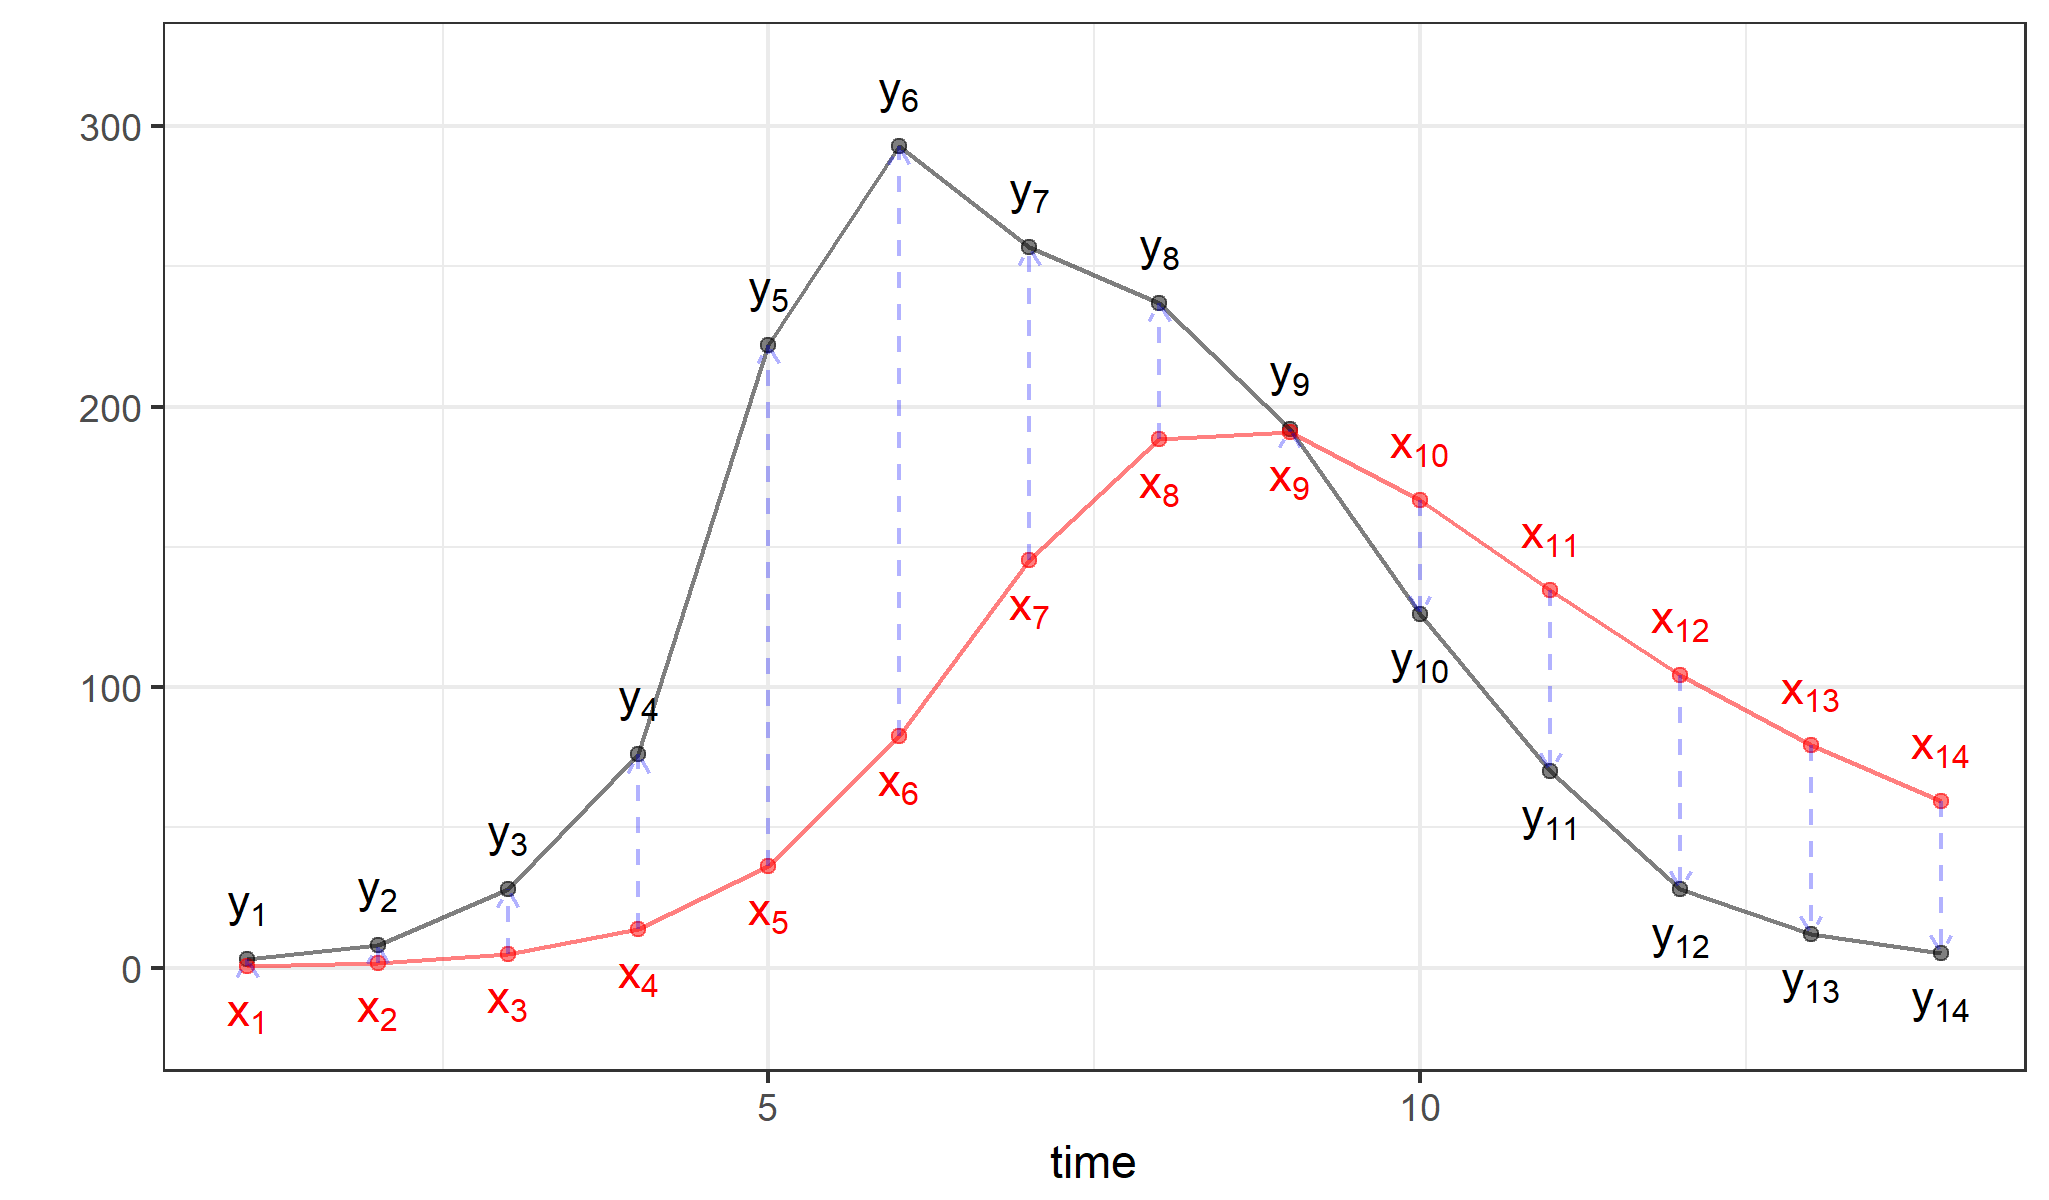
\includegraphics{figure/notes12-det-example-1} \end{center}

\begin{center}\rule{0.5\linewidth}{\linethickness}\end{center}

\begin{center}\rule{0.5\linewidth}{\linethickness}\end{center}

\subsection{Likelihood for stochastic models by direct
simulation}\label{likelihood-for-stochastic-models-by-direct-simulation}

\begin{itemize}
\item
  We can introduce the particle filter by first proposing a simpler
  method that usually doesn't work on anything but very short time
  series.
\item
  \textbf{Warning: this section is an example of what NOT to do!}
\item
  We can imagine using
  \href{./monteCarlo.html\#monte-carlo-integration}{Monte Carlo
  integration} for computing the likelihood of a state space model,
\end{itemize}

\begin{eqnarray}
\lik(\theta)
&=&
f_{Y_{1:N}}(\data{y_{1:N}}\params\theta)
\\
&=& \! \int_{x_{0:N}} \!\! f_{X_0}(x_0\params\theta)\prod_{n=1}^{N}\!f_{Y_n|X_n}(\data{y_n}\given x_n\params \theta)\, f_{X_n|X_{n-1}}(x_n|x_{n-1}\params\theta)\, dx_{0:N}.
\end{eqnarray}

\begin{itemize}
\item
  Specifically, if we have some probabilistic means of proposing
  trajectories for the unobserved state process, then we could just
  generate a large number of these and approximate \(\lik(\theta)\) by
  its Monte Carlo estimate.
\item
  Suppose we can generate \(J\) trajectories of length \(N\),
  \[\big\{ X_{n,j}, \; j=1\,\dots,J,\;  n=1,\dots,N\big\},\] from a
  joint density \(g_{X_{0:N}}(x_{0:N})\).
\item
  Let \(G_j\) denote the probability density for trajectory \(j\) under
  the model used to generate the trajectory, i.e.,
  \[G_{j}= g_{X_0}(X_{0,j})\prod_{n=1}^N g_{X_n|X_{n-1}}(X_{n,j}\given X_{n-1,j}).\]
\item
  Let \(F_j\) denote the probability density for trajectory \(j\) under
  our dynamic model, i.e.,
  \[F_{j}= f_{X_0}(X_{0,j}\params\theta)\prod_{n=1}^N f_{X_n|X_{n-1}}(X_{n,j}\given X_{n-1,j}\params\theta).\]
\item
  For each trajectory, we can compute the measurement likelihood of that
  trajectory, i.e., the measurement density

  \begin{eqnarray} 
  &&f_{Y_{1:N}|X_{1:N}}(\data{y_{1:N}}\given X_{1:N,j}\params\theta)
  \\
  &&\quad =\prod_{n=1}^{N} f_{Y_n|X_n}(\data{y_n}\given X_{n,j}\params\theta).
  \end{eqnarray}

  Then the \href{monteCarlo.html\#importance-sampling}{Monte Carlo
  importance sampling theorem} gives us
  \[\lik(\theta) \approx \frac{1}{J}\,\sum_{j=1}^{J}\!
  f_{Y_{1:N}|X_{1:N}}(\data{y_{1:N}}\given X_{1:N,j}\params\theta)
  \frac{F_j}{G_j}.\]
\item
  How shall we choose our trajectories? What is a good choice of the
  importance sampling proposal density, \(g_{X_{0:N}}(x_{0:N})\)?
\item
  A convenient choice is
  \[ g_{X_{0:N}}(x_{0:N}) = f_{X_{0:N}}(x_{0:N}\params\theta).\]
\item
  This choice of \(g_{X_{0:N}}(x_{0:N})\) means the numerator and
  denominator cancel in the importance sampling weights.
\item
  As a consequence, for this choice of \(g_{X_{0:N}}(x_{0:N})\) we never
  have to compute these weights.
\item
  This means, as long as we can simulate from the dynamic model,
  \(f_{X_{0:N}}(x_{0:N}\params\theta)\), we never have to evaluate this
  density.
\item
  We get the \textbf{plug-and-play} property that our algorithm depends
  on \texttt{rprocess} but does not require \texttt{dprocess}.
\item
  We see that, if we generate trajectories by simulation, all we have to
  do to get a Monte Carlo estimate of the likelihood is evaluate the
  measurement density of the data at each trajectory and average.
\item
  Let's go back to the boarding school influenza outbreak to see what
  this would look like.
\item
  Let's reconstruct the toy SIR model we were working with.
\end{itemize}

\begin{Shaded}
\begin{Highlighting}[]
\NormalTok{bsflu <-}\StringTok{ }\KeywordTok{read.table}\NormalTok{(}\StringTok{"bsflu_data.txt"}\NormalTok{)}

\NormalTok{sir_step <-}\StringTok{ }\KeywordTok{Csnippet}\NormalTok{(}\StringTok{"}
\StringTok{  double dN_SI = rbinom(S,1-exp(-Beta*I/N*dt));}
\StringTok{  double dN_IR = rbinom(I,1-exp(-gamma*dt));}
\StringTok{  S -= dN_SI;}
\StringTok{  I += dN_SI - dN_IR;}
\StringTok{  R += dN_IR;}
\StringTok{  H += dN_IR;}
\StringTok{"}\NormalTok{)}

\NormalTok{sir_init <-}\StringTok{ }\KeywordTok{Csnippet}\NormalTok{(}\StringTok{"}
\StringTok{  S = nearbyint(N)-1;}
\StringTok{  I = 1;}
\StringTok{  R = 0;}
\StringTok{  H = 0;}
\StringTok{"}\NormalTok{)}

\NormalTok{dmeas <-}\StringTok{ }\KeywordTok{Csnippet}\NormalTok{(}\StringTok{"lik = dbinom(B,H,rho,give_log);"}\NormalTok{)}
\NormalTok{rmeas <-}\StringTok{ }\KeywordTok{Csnippet}\NormalTok{(}\StringTok{"B = rbinom(H,rho);"}\NormalTok{)}

\KeywordTok{pomp}\NormalTok{(bsflu,}\DataTypeTok{times=}\StringTok{"day"}\NormalTok{,}\DataTypeTok{t0=}\DecValTok{0}\NormalTok{,}
     \DataTypeTok{rprocess=}\KeywordTok{euler.sim}\NormalTok{(sir_step,}\DataTypeTok{delta.t=}\DecValTok{1}\OperatorTok{/}\DecValTok{5}\NormalTok{),}
     \DataTypeTok{initializer=}\NormalTok{sir_init,}\DataTypeTok{rmeasure=}\NormalTok{rmeas,}\DataTypeTok{dmeasure=}\NormalTok{dmeas,}
     \DataTypeTok{zeronames=}\StringTok{"H"}\NormalTok{,}\DataTypeTok{statenames=}\KeywordTok{c}\NormalTok{(}\StringTok{"H"}\NormalTok{,}\StringTok{"S"}\NormalTok{,}\StringTok{"I"}\NormalTok{,}\StringTok{"R"}\NormalTok{),}
     \DataTypeTok{paramnames=}\KeywordTok{c}\NormalTok{(}\StringTok{"Beta"}\NormalTok{,}\StringTok{"gamma"}\NormalTok{,}\StringTok{"rho"}\NormalTok{,}\StringTok{"N"}\NormalTok{),}
     \DataTypeTok{cdir =} \KeywordTok{getwd}\NormalTok{()) ->}\StringTok{ }\NormalTok{sir}
\end{Highlighting}
\end{Shaded}

\begin{itemize}
\tightlist
\item
  Let's generate a bunch of simulated trajectories at some particular
  point in parameter space.
\end{itemize}

\begin{Shaded}
\begin{Highlighting}[]
\KeywordTok{simulate}\NormalTok{(sir,}\DataTypeTok{params=}\KeywordTok{c}\NormalTok{(}\DataTypeTok{Beta=}\DecValTok{2}\NormalTok{,}\DataTypeTok{gamma=}\DecValTok{1}\NormalTok{,}\DataTypeTok{rho=}\FloatTok{0.5}\NormalTok{,}\DataTypeTok{N=}\DecValTok{2600}\NormalTok{),}
         \DataTypeTok{nsim=}\DecValTok{10000}\NormalTok{,}\DataTypeTok{states=}\OtherTok{TRUE}\NormalTok{) ->}\StringTok{ }\NormalTok{x}
\KeywordTok{matplot}\NormalTok{(}\KeywordTok{time}\NormalTok{(sir),}\KeywordTok{t}\NormalTok{(x[}\StringTok{"H"}\NormalTok{,}\DecValTok{1}\OperatorTok{:}\DecValTok{50}\NormalTok{,]),}\DataTypeTok{type=}\StringTok{'l'}\NormalTok{,}\DataTypeTok{lty=}\DecValTok{1}\NormalTok{,}
        \DataTypeTok{xlab=}\StringTok{"time"}\NormalTok{,}\DataTypeTok{ylab=}\StringTok{"H"}\NormalTok{,}\DataTypeTok{bty=}\StringTok{'l'}\NormalTok{,}\DataTypeTok{col=}\StringTok{'blue'}\NormalTok{)}
\KeywordTok{lines}\NormalTok{(}\KeywordTok{time}\NormalTok{(sir),}\KeywordTok{obs}\NormalTok{(sir,}\StringTok{"B"}\NormalTok{),}\DataTypeTok{lwd=}\DecValTok{2}\NormalTok{,}\DataTypeTok{col=}\StringTok{'black'}\NormalTok{)}
\end{Highlighting}
\end{Shaded}

\begin{center}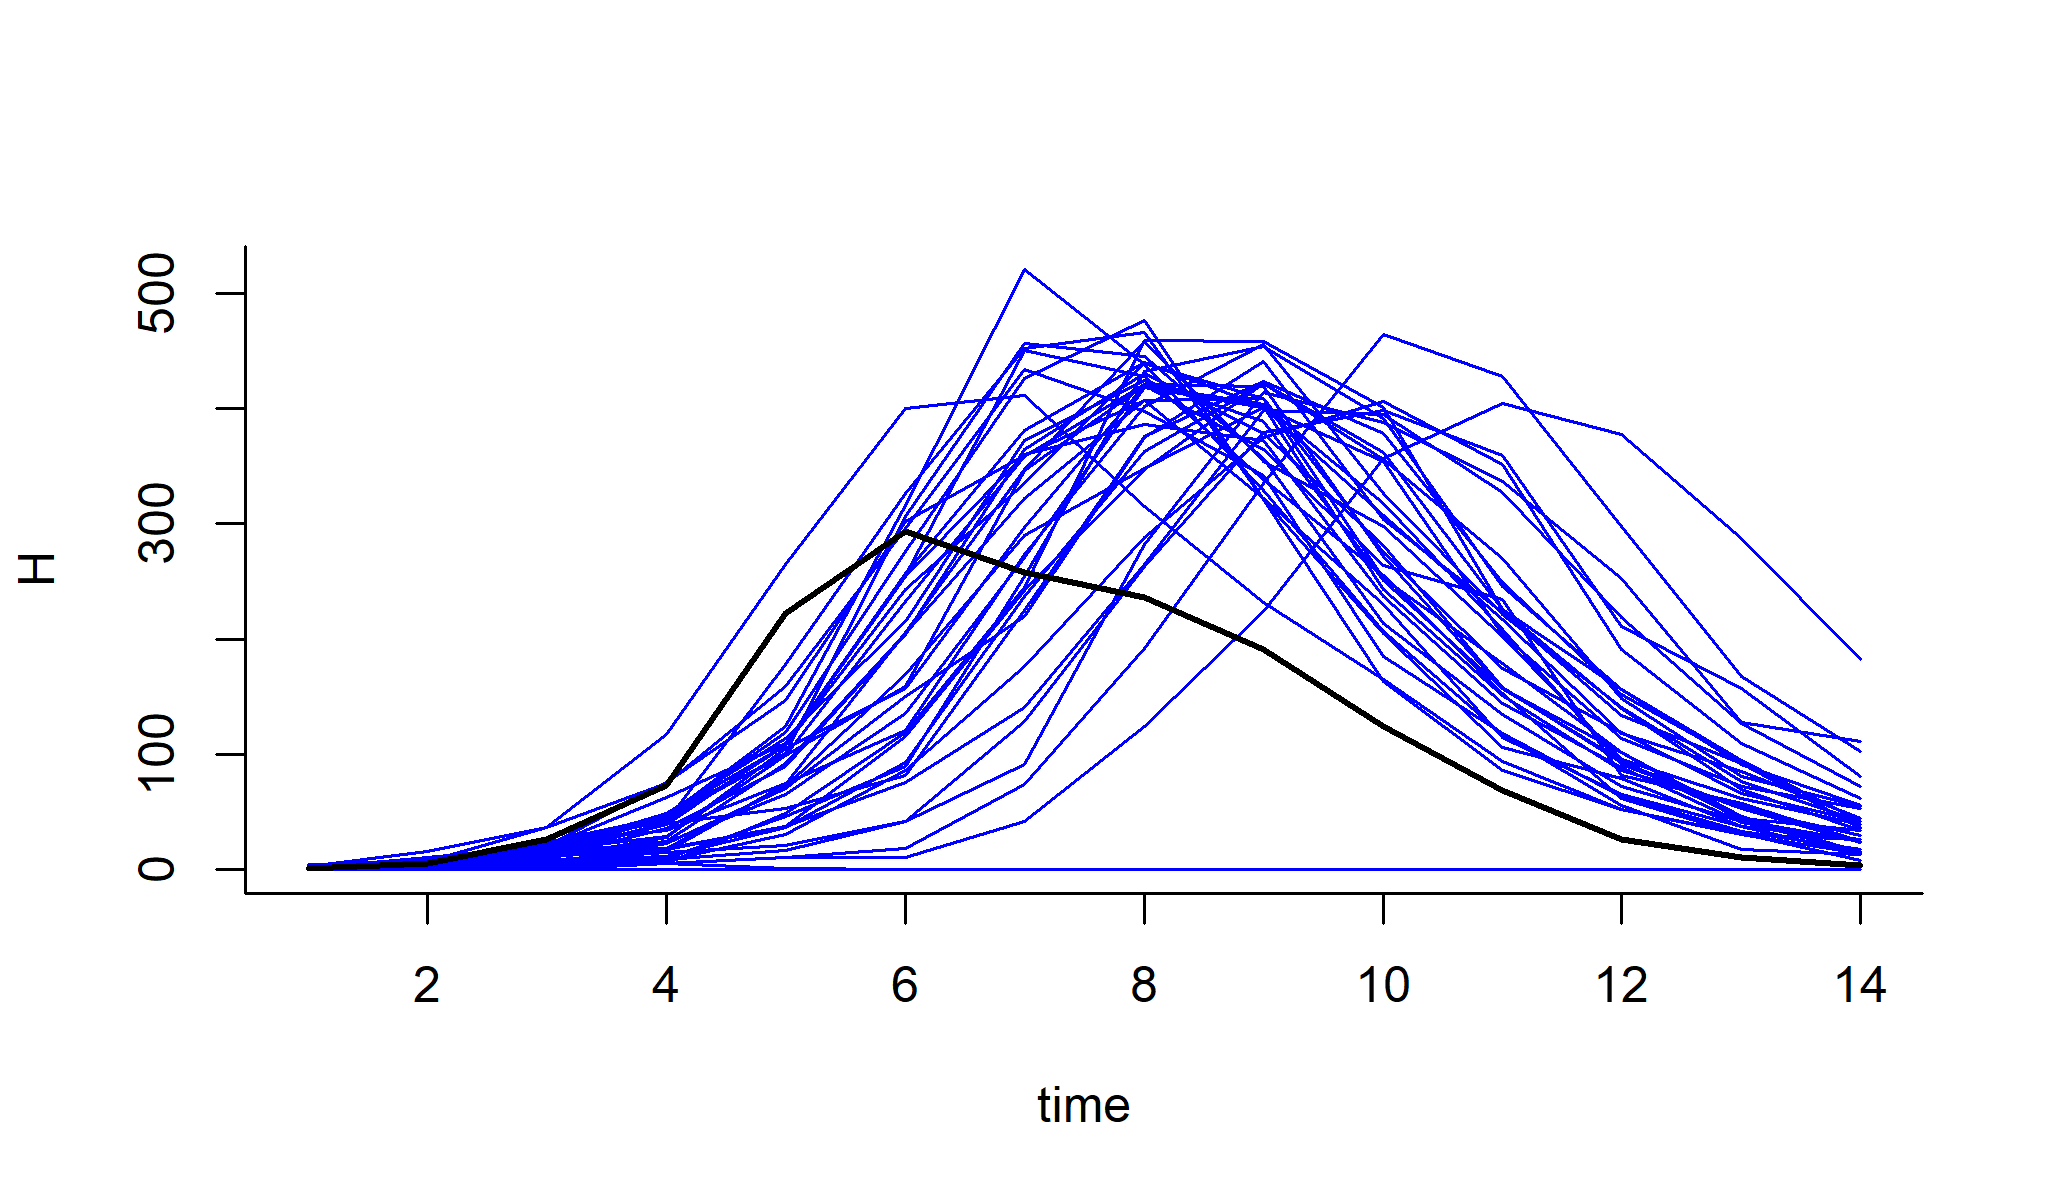
\includegraphics{figure/notes12-bbs-mc-like-2-1} \end{center}

\begin{itemize}
\tightlist
\item
  We can use the function \texttt{dmeasure} to evaluate the log
  likelihood of the data given the states, the model, and the
  parameters:
\end{itemize}

\begin{Shaded}
\begin{Highlighting}[]
\NormalTok{ell <-}\StringTok{ }\KeywordTok{dmeasure}\NormalTok{(sir,}\DataTypeTok{y=}\KeywordTok{obs}\NormalTok{(sir),}\DataTypeTok{x=}\NormalTok{x,}\DataTypeTok{times=}\KeywordTok{time}\NormalTok{(sir),}\DataTypeTok{log=}\OtherTok{TRUE}\NormalTok{,}
                \DataTypeTok{params=}\KeywordTok{c}\NormalTok{(}\DataTypeTok{Beta=}\DecValTok{2}\NormalTok{,}\DataTypeTok{gamma=}\DecValTok{1}\NormalTok{,}\DataTypeTok{rho=}\FloatTok{0.5}\NormalTok{,}\DataTypeTok{N=}\DecValTok{2600}\NormalTok{))}
\KeywordTok{dim}\NormalTok{(ell)}
\end{Highlighting}
\end{Shaded}

\begin{verbatim}
## [1] 10000    14
\end{verbatim}

\begin{itemize}
\tightlist
\item
  According to the equation above, we should sum up the log likelihoods
  across time:
\end{itemize}

\begin{Shaded}
\begin{Highlighting}[]
\NormalTok{ell <-}\StringTok{ }\KeywordTok{apply}\NormalTok{(ell,}\DecValTok{1}\NormalTok{,sum); }\KeywordTok{summary}\NormalTok{(}\KeywordTok{exp}\NormalTok{(ell)); }\KeywordTok{logmeanexp}\NormalTok{(ell,}\DataTypeTok{se=}\OtherTok{TRUE}\NormalTok{)}
\end{Highlighting}
\end{Shaded}

\begin{verbatim}
##      Min.   1st Qu.    Median      Mean   3rd Qu.      Max. 
##  0.00e+00  0.00e+00  0.00e+00 5.37e-106  0.00e+00 5.37e-102
\end{verbatim}

\begin{verbatim}
##                    se 
## -242.39328   16.09139
\end{verbatim}

\begin{itemize}
\item
  The likelihood appears to be very low, but the error in the estimate
  is very high and therefore the estimated likelihood is very imprecise.
\item
  We are going to need very many simulations to get an estimate of the
  likelihood sufficiently precise to be of any use in parameter
  estimation or model selection.
\item
  What's the problem? Essentially, far too many of the trajectories
  don't pass near the data. Moreover, once a trajectory diverges from
  the data, it almost never comes back.
\item
  This is a consequence of the fact that we are proposing trajectories
  in a way that is completely unconditional on the data.
\item
  The problem will only get worse with longer data sets!
\end{itemize}

\hypertarget{the-particle-filter}{\subsection{The particle
filter}\label{the-particle-filter}}

\begin{itemize}
\item
  Fortunately, we can compute the likelihood for a POMP model by a much
  more efficient algorithm than direct Monte Carlo integration.
\item
  We proceed by factorizing the likelihood in a different way:
\end{itemize}

\begin{eqnarray}
\lik(\theta)&=&f_{Y_{1:N}}(y^*_{1:N}\params \theta)
\\
&=&
\prod_{n}\,f_{Y_N|Y_{1:N-1}}(y^*_n|y^*_{1:n-1}\params\theta) 
\\
&=&
\prod_{n}\,\int f_{Y_n|X_n}(y^*_n|x_n\params\theta)\,f_{X_n|Y_{1:n-1}}(x_n|y^*_{1:n-1}\params\theta)\, dx_{n}.
\end{eqnarray}

\begin{itemize}
\tightlist
\item
  The Markov property leads to the prediction formula:
\end{itemize}

\begin{eqnarray}
&&f_{X_n|Y_{1:n-1}}(x_n|y^*_{1:n-1}\params \theta) 
\\
&&\quad
= \int_{x_{n-1}} \! f_{X_n|X_{n-1}}(x_n|x_{n-1}\params\theta)\, f_{X_{n-1}|Y_{1:n-1}}(x_{n-1}\given y^*_{1:n-1}\params \theta) \, dx_{n-1}.
\end{eqnarray}

\begin{itemize}
\tightlist
\item
  Bayes' theorem gives the filtering formula:
\end{itemize}

\begin{eqnarray}
&&f_{X_n|Y_{1:n}}(x_n|y^*_{1:n}\params \theta)
\\
&&\quad = f_{X_n|Y_n,Y_{1:n-1}}(x_n|y^*_n,y^*_{1:n-1}\params \theta) 
\\
&&\quad =\frac{f_{Y_n|X_n}(y^*_{n}|x_{n}\params\theta)\,f_{X_n|Y_{1:n-1}}(x_{n}|y^*_{1:n-1}\params\theta)}{\int
f_{Y_n|X_n}(y^*_{n}|u_{n}\params\theta)\,f_{X_n|Y_{1:n-1}}(u_{n}|y^*_{1:n-1}\params\theta)\, du_n}.
\end{eqnarray}

\begin{itemize}
\item
  This suggests that we keep track of two key distributions. We'll refer
  to the distribution of \(X_n | Y_{1:n-1}\equals y^*_{1:n-1}\) as the
  \textbf{prediction distribution} at time \(t_n\) and the distribution
  of \(X_{n} | Y_{1:n}\equals y^*_{1:n}\) as the \textbf{filtering
  distribution} at time \(t_n\).
\item
  Let's use Monte Carlo techniques to estimate the integrals in the
  prediction and filtering recursion equations.
\item
  Consider the following Monte Carlo scheme:
\end{itemize}

\begin{enumerate}
\def\labelenumi{\arabic{enumi}.}
\item
  Suppose \(X_{n-1,j}^{F}\), \(j=1,\dots,J\) is a set of \(J\) points
  drawn from the filtering distribution at time \(n-1\).
\item
  We obtain a sample \(X_{n,j}^{P}\) of points drawn from the prediction
  distribution at time \(t\) by simply simulating the process model:
  \[X_{n,j}^{P} \sim \mathrm{process}(X_{n-1,j}^{F},\theta), \qquad j=1,\dots,J.\]
\item
  Having obtained \(x_{n,j}^{P}\), we obtain a sample of points from the
  filtering distribution at time \(t_n\) by \emph{resampling} from
  \(\big\{X_{n,j}^{P},j\in 1:J\big\}\) with weights
  \[w_{n,j}=f_{Y_n|X_n}(y^*_{n}|X^P_{n,j}\params\theta).\]
\item
  The Monte Carlo principle tells us that the conditional likelihood

  \begin{eqnarray}
  \lik_n(\theta) &=& f_{Y_n|Y_{1:n-1}}(y^*_n|y^*_{1:n-1}\params\theta)
  \\
  &=& 
  \int
  f_{Y_n|X_n}(y^*_{n}|x_{n}\params\theta)\,f_{X_n|Y_{1:n-1}}(x_{n}|y^*_{1:n-1}\params\theta)\, dx_n
  \end{eqnarray}
\end{enumerate}

is approximated by
\[\hat\lik_n(\theta)  \approx \frac{1}{N}\,\sum_j\, f_{Y_n|X_n}(y^*_{n}|X_{n,j}^{P}\params\theta).\]

\begin{enumerate}
\def\labelenumi{\arabic{enumi}.}
\setcounter{enumi}{4}
\item
  We can iterate this procedure through the data, one step at a time,
  alternately simulating and resampling, until we reach \(n=N\).
\item
  The full log likelihood then has approximation

  \begin{eqnarray}\loglik(\theta) 
  &=& \log{\lik(\theta)} 
  \\
  &=& \sum_n \log{\lik_n(\theta)}
  \\
  &\approx& \sum_n\log\hat\lik_n(\theta).
  \end{eqnarray}
\end{enumerate}

\begin{itemize}
\item
  The above procedure is known as the \textbf{sequential Monte Carlo}
  (SMC) algorithm or the \textbf{particle filter}.
\item
  Good references for further reading include Kitagawa (1987),
  Arulampalam et al. (2002) and the book edited by Doucet et al. (2001).
\end{itemize}

\subsection{\texorpdfstring{Sequential Monte Carlo in
\textbf{pomp}}{Sequential Monte Carlo in pomp}}\label{sequential-monte-carlo-in-pomp}

\begin{itemize}
\tightlist
\item
  Here, we'll get some practical experience with the particle filter,
  and the likelihood function, in the context of our influenza-outbreak
  case study.
\end{itemize}

\begin{Shaded}
\begin{Highlighting}[]
\NormalTok{sims <-}\StringTok{ }\KeywordTok{simulate}\NormalTok{(sir,}\DataTypeTok{params=}\KeywordTok{c}\NormalTok{(}\DataTypeTok{Beta=}\DecValTok{2}\NormalTok{,}\DataTypeTok{gamma=}\DecValTok{1}\NormalTok{,}\DataTypeTok{rho=}\FloatTok{0.8}\NormalTok{,}\DataTypeTok{N=}\DecValTok{2600}\NormalTok{),}\DataTypeTok{nsim=}\DecValTok{20}\NormalTok{,}
                 \DataTypeTok{as.data.frame=}\OtherTok{TRUE}\NormalTok{,}\DataTypeTok{include.data=}\OtherTok{TRUE}\NormalTok{)}

\KeywordTok{ggplot}\NormalTok{(sims,}\DataTypeTok{mapping=}\KeywordTok{aes}\NormalTok{(}\DataTypeTok{x=}\NormalTok{time,}\DataTypeTok{y=}\NormalTok{B,}\DataTypeTok{group=}\NormalTok{sim,}\DataTypeTok{color=}\NormalTok{sim}\OperatorTok{==}\StringTok{"data"}\NormalTok{))}\OperatorTok{+}
\StringTok{  }\KeywordTok{geom_line}\NormalTok{()}\OperatorTok{+}\KeywordTok{guides}\NormalTok{(}\DataTypeTok{color=}\OtherTok{FALSE}\NormalTok{)}
\end{Highlighting}
\end{Shaded}

\begin{center}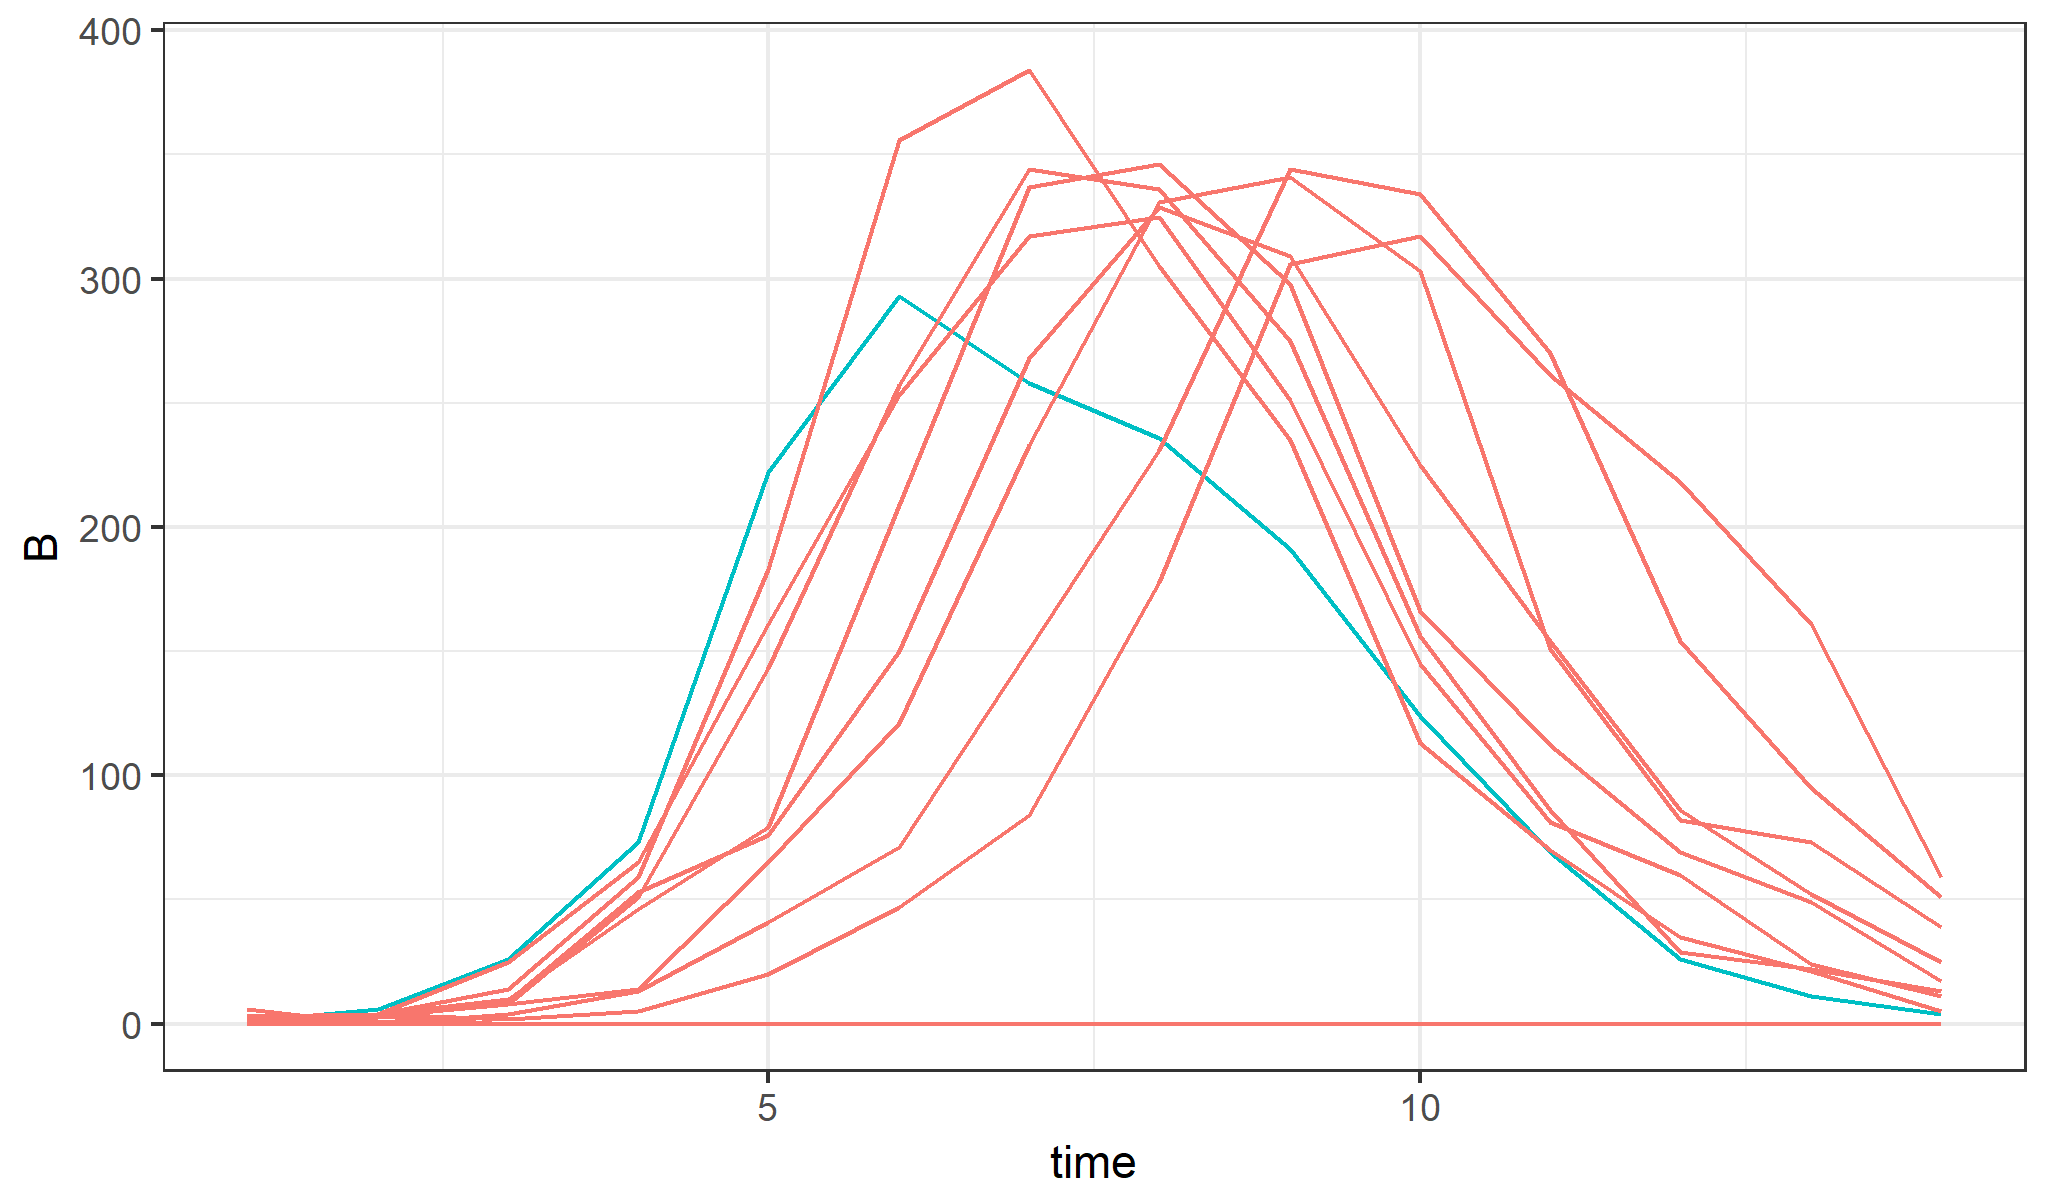
\includegraphics{figure/notes12-sir-sim1-1} \end{center}

\begin{itemize}
\tightlist
\item
  In \textbf{pomp}, the basic particle filter is implemented in the
  command \texttt{pfilter}. We must choose the number of particles to
  use by setting the \texttt{Np} argument.
\end{itemize}

\begin{Shaded}
\begin{Highlighting}[]
\NormalTok{pf <-}\StringTok{ }\KeywordTok{pfilter}\NormalTok{(sir,}\DataTypeTok{Np=}\DecValTok{5000}\NormalTok{,}\DataTypeTok{params=}\KeywordTok{c}\NormalTok{(}\DataTypeTok{Beta=}\DecValTok{2}\NormalTok{,}\DataTypeTok{gamma=}\DecValTok{1}\NormalTok{,}\DataTypeTok{rho=}\FloatTok{0.8}\NormalTok{,}\DataTypeTok{N=}\DecValTok{2600}\NormalTok{))}
\KeywordTok{logLik}\NormalTok{(pf)}
\end{Highlighting}
\end{Shaded}

\begin{verbatim}
## [1] -69.73054
\end{verbatim}

\begin{itemize}
\tightlist
\item
  We can run a few particle filters to get an estimate of the Monte
  Carlo variability:
\end{itemize}

\begin{Shaded}
\begin{Highlighting}[]
\NormalTok{pf <-}\StringTok{ }\KeywordTok{replicate}\NormalTok{(}\DecValTok{10}\NormalTok{,}\KeywordTok{pfilter}\NormalTok{(sir,}\DataTypeTok{Np=}\DecValTok{5000}\NormalTok{,}\DataTypeTok{params=}\KeywordTok{c}\NormalTok{(}\DataTypeTok{Beta=}\DecValTok{2}\NormalTok{,}\DataTypeTok{gamma=}\DecValTok{1}\NormalTok{,}\DataTypeTok{rho=}\FloatTok{0.8}\NormalTok{,}\DataTypeTok{N=}\DecValTok{2600}\NormalTok{)))}
\NormalTok{ll <-}\StringTok{ }\KeywordTok{sapply}\NormalTok{(pf,logLik); ll}
\end{Highlighting}
\end{Shaded}

\begin{verbatim}
##  [1] -76.60686 -82.19224 -80.33033 -88.14655 -71.78196 -71.64952 -84.32846
##  [8] -82.05719 -76.90641 -77.36237
\end{verbatim}

\begin{Shaded}
\begin{Highlighting}[]
\KeywordTok{logmeanexp}\NormalTok{(ll,}\DataTypeTok{se=}\OtherTok{TRUE}\NormalTok{)}
\end{Highlighting}
\end{Shaded}

\begin{verbatim}
##                      se 
## -73.3146129   0.8277326
\end{verbatim}

\begin{itemize}
\item
  A theoretical property of the particle filter is that it gives us an
  unbiased Monte Carlo estimate of the likelihood.
\item
  This theoretical property, combined with
  \href{https://en.wikipedia.org/wiki/Jensen\%27s_inequality}{Jensen's
  inequality} and the observation that \(\log(x)\) is a concave
  function, ensures that the average of the log likelihoods from many
  particle filter replications will have negative bias as a Monte Carlo
  estimator of the log likelihood.
\item
  We've been careful to avoid this bias in the code above, by using
  \texttt{logmeanexp} to average the likelihood estimates on the natural
  scale not the logarithmic scale.
\end{itemize}

\begin{center}\rule{0.5\linewidth}{\linethickness}\end{center}

\begin{center}\rule{0.5\linewidth}{\linethickness}\end{center}

\subsection{The graph of the likelihood function: The likelihood
surface}\label{the-graph-of-the-likelihood-function-the-likelihood-surface}

\begin{itemize}
\item
  Intuitively, it can be helpful to think of the geometric surface
  defined by the likelihood function.
\item
  If \(\Theta\) is two-dimensional, then the surface \(\ell(\theta)\)
  has features like a landscape.

  \begin{itemize}
  \item
    Local maxima of \(\ell(\theta)\) are peaks
  \item
    local minima are valleys
  \item
    peaks may be separated by a valley or may be joined by a ridge. If
    you go along the ridge, you may be able to go from one peak to the
    other without losing much elevation. Narrow ridges can be easy to
    fall off, and hard to get back on to.
  \end{itemize}
\item
  In higher dimensions, one can still think of peaks and valleys and
  ridges. However, as the dimension increases it quickly becomes hard to
  imagine the surface.
\item
  To get an idea of what the likelihood surface looks like in the
  neighborhood of the default parameter set supplied by \texttt{sir}, we
  can construct a \textbf{likelihood slice}.
\item
  We'll make slices in the \(\beta\) and \(\gamma\) directions. Both
  slices will pass through the default parameter set.
\end{itemize}

\begin{Shaded}
\begin{Highlighting}[]
\KeywordTok{sliceDesign}\NormalTok{(}
  \KeywordTok{c}\NormalTok{(}\DataTypeTok{Beta=}\DecValTok{2}\NormalTok{,}\DataTypeTok{gamma=}\DecValTok{1}\NormalTok{,}\DataTypeTok{rho=}\FloatTok{0.8}\NormalTok{,}\DataTypeTok{N=}\DecValTok{2600}\NormalTok{),}
  \DataTypeTok{Beta=}\KeywordTok{rep}\NormalTok{(}\KeywordTok{seq}\NormalTok{(}\DataTypeTok{from=}\FloatTok{0.5}\NormalTok{,}\DataTypeTok{to=}\DecValTok{4}\NormalTok{,}\DataTypeTok{length=}\DecValTok{40}\NormalTok{),}\DataTypeTok{each=}\DecValTok{3}\NormalTok{),}
  \DataTypeTok{gamma=}\KeywordTok{rep}\NormalTok{(}\KeywordTok{seq}\NormalTok{(}\DataTypeTok{from=}\FloatTok{0.5}\NormalTok{,}\DataTypeTok{to=}\DecValTok{2}\NormalTok{,}\DataTypeTok{length=}\DecValTok{40}\NormalTok{),}\DataTypeTok{each=}\DecValTok{3}\NormalTok{)) ->}\StringTok{ }\NormalTok{p}

\KeywordTok{require}\NormalTok{(foreach)}
\KeywordTok{require}\NormalTok{(doMC)}

\KeywordTok{registerDoMC}\NormalTok{(}\DataTypeTok{cores=}\DecValTok{5}\NormalTok{)        }
\NormalTok{## number of cores }
\NormalTok{## usually the number of cores on your machine, or slightly smaller}

\KeywordTok{set.seed}\NormalTok{(998468235L,}\DataTypeTok{kind=}\StringTok{"L'Ecuyer"}\NormalTok{)}
\NormalTok{mcopts <-}\StringTok{ }\KeywordTok{list}\NormalTok{(}\DataTypeTok{preschedule=}\OtherTok{FALSE}\NormalTok{,}\DataTypeTok{set.seed=}\OtherTok{TRUE}\NormalTok{)}

\KeywordTok{foreach}\NormalTok{ (}\DataTypeTok{theta=}\KeywordTok{iter}\NormalTok{(p,}\StringTok{"row"}\NormalTok{),}\DataTypeTok{.combine=}\NormalTok{rbind,}
         \DataTypeTok{.inorder=}\OtherTok{FALSE}\NormalTok{,}\DataTypeTok{.options.multicore=}\NormalTok{mcopts) }\OperatorTok\StringTok{ }
\StringTok{ }\NormalTok{\{}
   \KeywordTok{pfilter}\NormalTok{(sir,}\DataTypeTok{params=}\KeywordTok{unlist}\NormalTok{(theta),}\DataTypeTok{Np=}\DecValTok{5000}\NormalTok{) ->}\StringTok{ }\NormalTok{pf}
\NormalTok{   theta}\OperatorTok{$}\NormalTok{loglik <-}\StringTok{ }\KeywordTok{logLik}\NormalTok{(pf)}
\NormalTok{   theta}
\NormalTok{ \} ->}\StringTok{ }\NormalTok{p}
\end{Highlighting}
\end{Shaded}

\begin{itemize}
\tightlist
\item
  You can see from the code what is meant by a likelihood slice.
\end{itemize}

\begin{center}\rule{0.5\linewidth}{\linethickness}\end{center}

\begin{center}\rule{0.5\linewidth}{\linethickness}\end{center}

\subsubsection{Exercise: Write down the definition of a likelihood slice
in mathematical
notation.}\label{exercise-write-down-the-definition-of-a-likelihood-slice-in-mathematical-notation.}

\subsubsection{Exercise: Note that a likelihood slice is different from
a likelihood
profile}\label{exercise-note-that-a-likelihood-slice-is-different-from-a-likelihood-profile}

\begin{itemize}
\item
  What is the difference between a likelihood slice and a profile from a
  computational perspective?
\item
  What is the difference between the statistical interpretation of a
  likelihood slice and a profile. For example, compare their roles in
  constructing confidence intervals and hypothesis tests.
\item
  What is the purpose of computing a likelihood slice? What is the
  purpose of computing a likelihood profile?
\end{itemize}

\begin{center}\rule{0.5\linewidth}{\linethickness}\end{center}

\begin{center}\rule{0.5\linewidth}{\linethickness}\end{center}

\begin{itemize}
\item
  Note that the slice computation used the \textbf{foreach} package with
  the multicore backend (\textbf{doMC}) to parallelize these
  computations.
\item
  To ensure that we have high-quality random numbers in each parallel
  \emph{R} session, we use a parallel random number generator. Notice
  the specification \texttt{kind="L\textquotesingle{}Ecuyer"} when we
  set the seed for the random number generator, and the specification
  \texttt{.options.multicore=mcopts} for \texttt{foreach}, the parallel
  for loop
\item
  Now, we can plot the likelihood slices:
\end{itemize}

\begin{Shaded}
\begin{Highlighting}[]
\KeywordTok{foreach}\NormalTok{ (}\DataTypeTok{v=}\KeywordTok{c}\NormalTok{(}\StringTok{"Beta"}\NormalTok{,}\StringTok{"gamma"}\NormalTok{)) }\OperatorTok\StringTok{ }
\NormalTok{\{}
\NormalTok{  x <-}\StringTok{ }\KeywordTok{subset}\NormalTok{(p,slice}\OperatorTok{==}\NormalTok{v)}
  \KeywordTok{plot}\NormalTok{(x[[v]],x}\OperatorTok{$}\NormalTok{loglik,}\DataTypeTok{xlab=}\NormalTok{v,}\DataTypeTok{ylab=}\StringTok{"loglik"}\NormalTok{)}
\NormalTok{\}}
\end{Highlighting}
\end{Shaded}

\begin{center}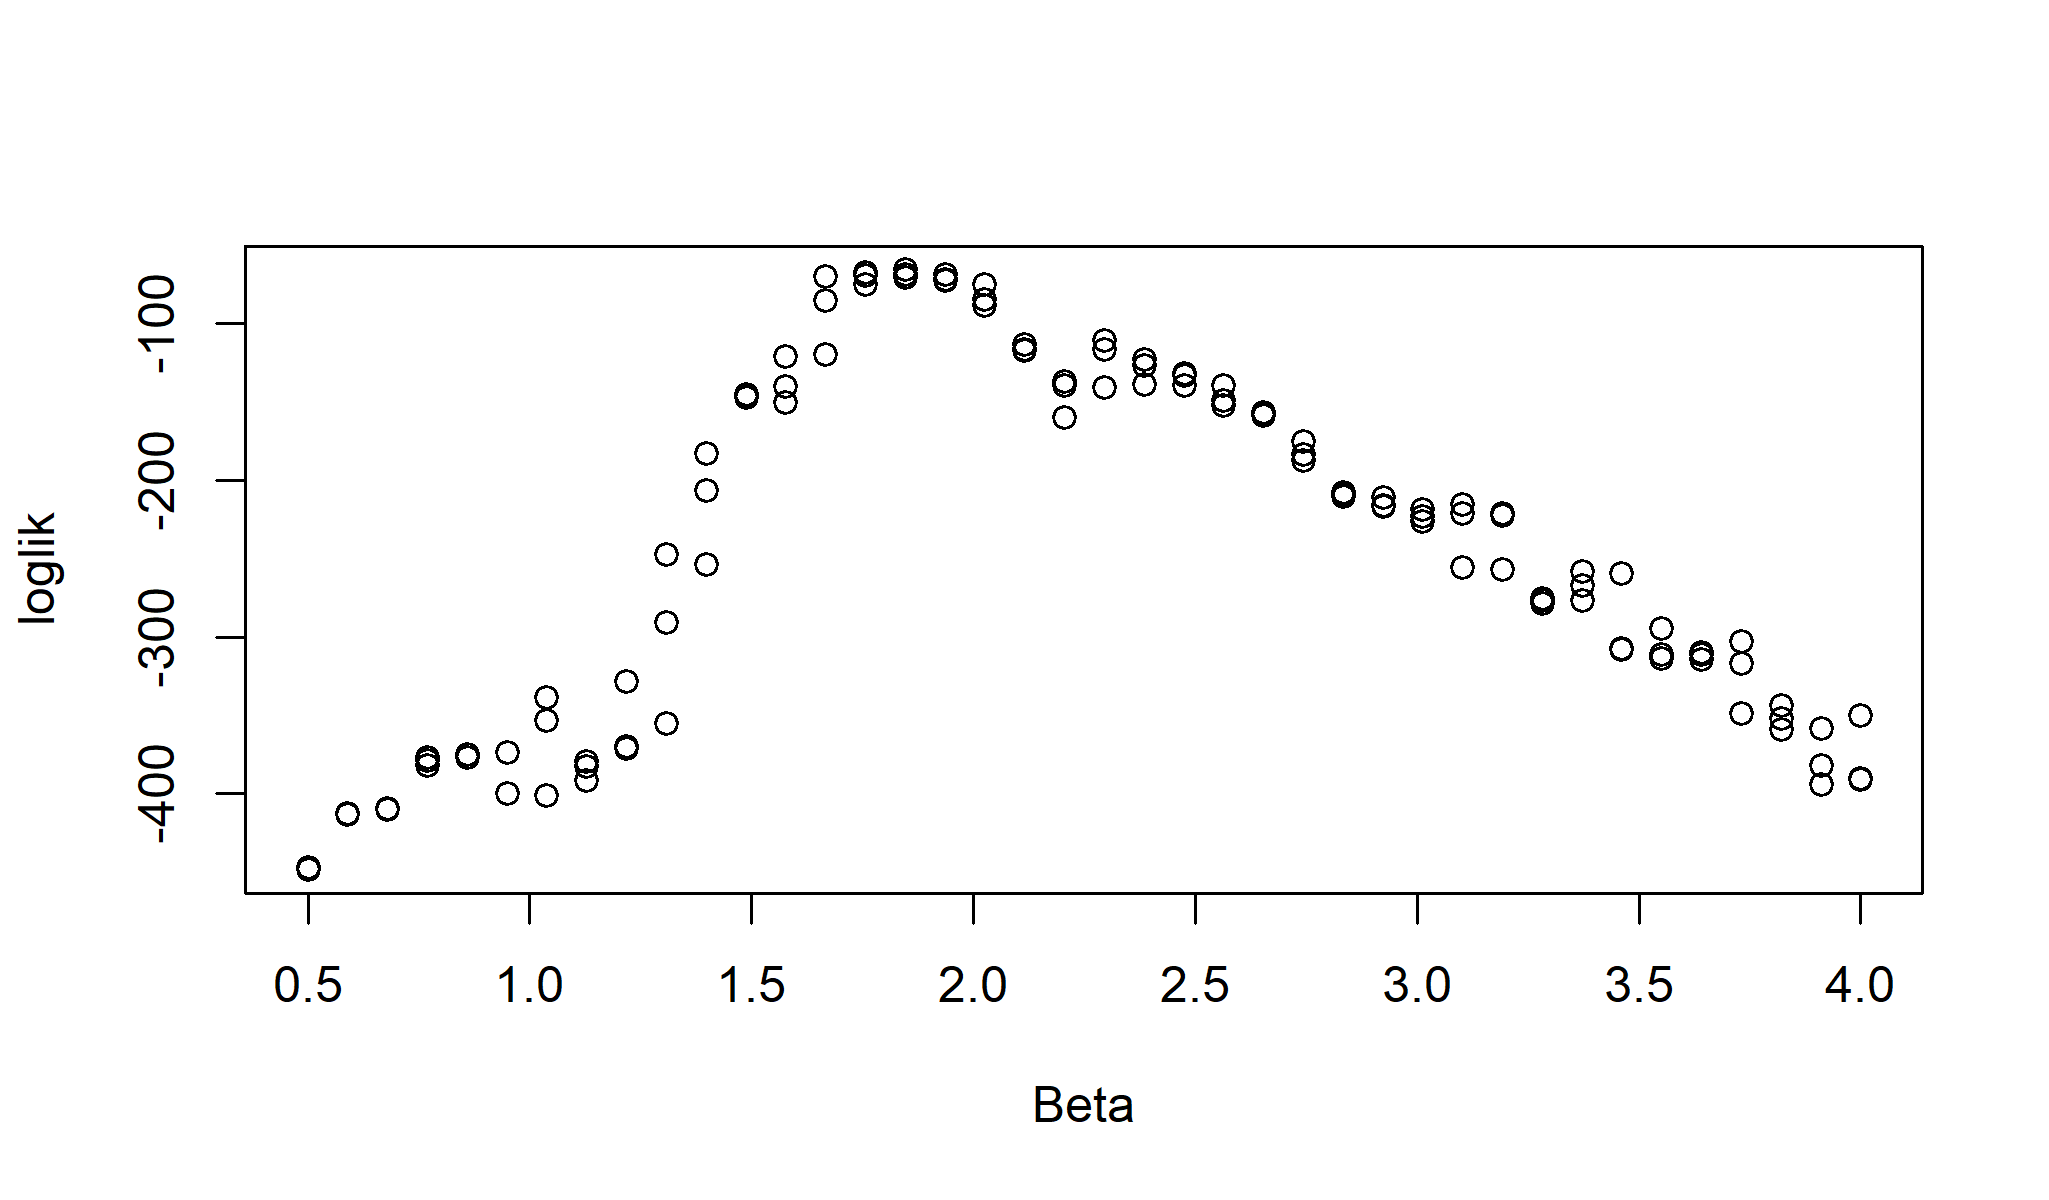
\includegraphics{figure/notes12-sir-like-slice-plot-1} \end{center}

\begin{center}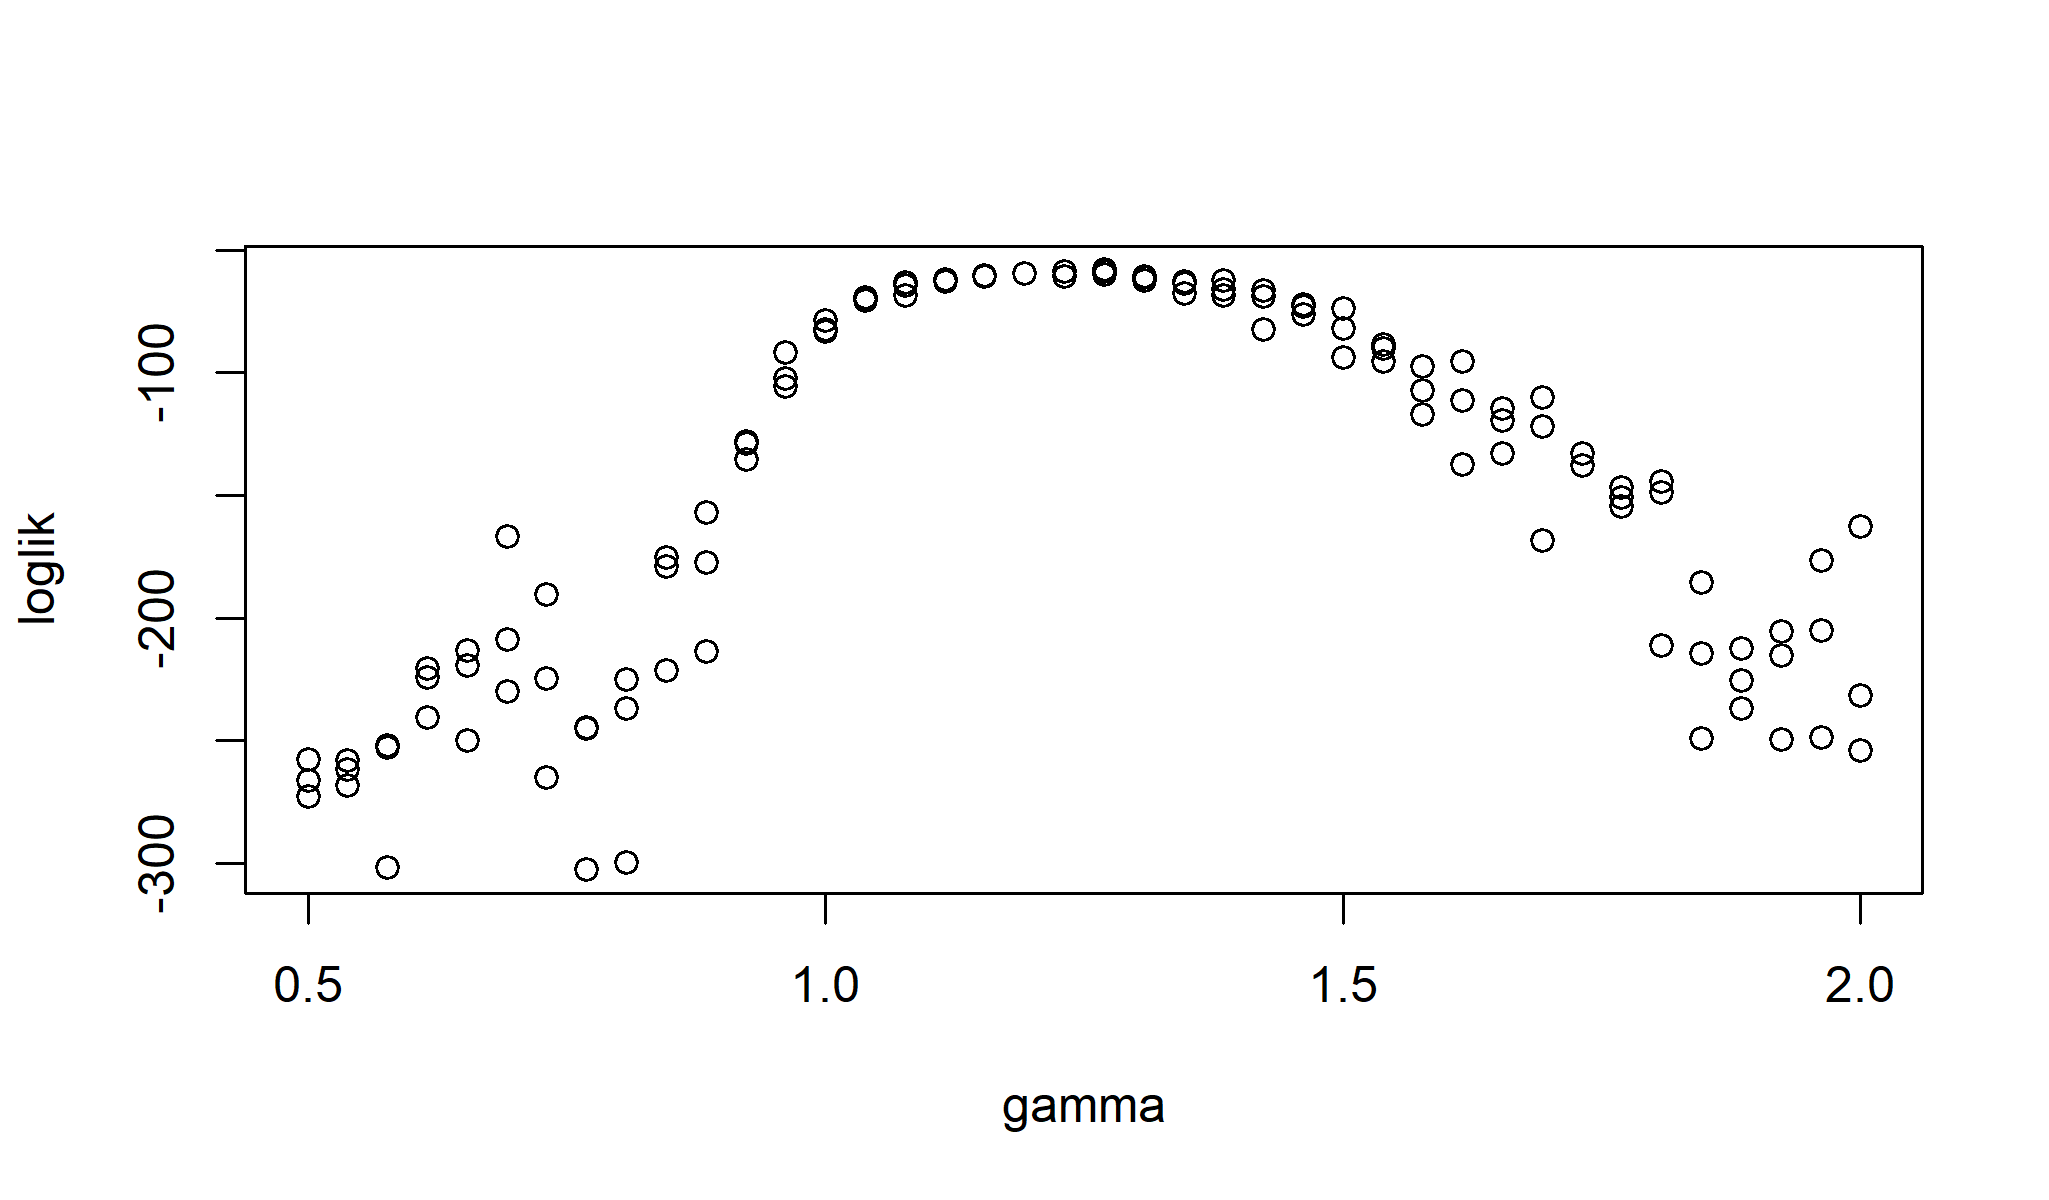
\includegraphics{figure/notes12-sir-like-slice-plot-2} \end{center}

\begin{center}\rule{0.5\linewidth}{\linethickness}\end{center}

\subsubsection{Exercise: Likelihood
slices}\label{exercise-likelihood-slices}

Add likelihood slices along the \(\rho\) direction.

\begin{center}\rule{0.5\linewidth}{\linethickness}\end{center}

Slices offer a very limited perspective on the geometry of the
likelihood surface. With just two parameters, we can evaluate the
likelihood at a grid of points and visualize the surface directly.

\begin{Shaded}
\begin{Highlighting}[]
\KeywordTok{expand.grid}\NormalTok{(}\DataTypeTok{Beta=}\KeywordTok{seq}\NormalTok{(}\DataTypeTok{from=}\DecValTok{1}\NormalTok{,}\DataTypeTok{to=}\DecValTok{4}\NormalTok{,}\DataTypeTok{length=}\DecValTok{50}\NormalTok{),}
            \DataTypeTok{gamma=}\KeywordTok{seq}\NormalTok{(}\DataTypeTok{from=}\FloatTok{0.7}\NormalTok{,}\DataTypeTok{to=}\DecValTok{3}\NormalTok{,}\DataTypeTok{length=}\DecValTok{50}\NormalTok{),}
            \DataTypeTok{rho=}\FloatTok{0.8}\NormalTok{,}
            \DataTypeTok{N=}\DecValTok{2600}\NormalTok{) ->}\StringTok{ }\NormalTok{p}

\KeywordTok{foreach}\NormalTok{ (}\DataTypeTok{theta=}\KeywordTok{iter}\NormalTok{(p,}\StringTok{"row"}\NormalTok{),}\DataTypeTok{.combine=}\NormalTok{rbind,}
         \DataTypeTok{.inorder=}\OtherTok{FALSE}\NormalTok{,}\DataTypeTok{.options.multicore=}\NormalTok{mcopts) }\OperatorTok\StringTok{ }
\StringTok{ }\NormalTok{\{}
   \KeywordTok{pfilter}\NormalTok{(sir,}\DataTypeTok{params=}\KeywordTok{unlist}\NormalTok{(theta),}\DataTypeTok{Np=}\DecValTok{5000}\NormalTok{) ->}\StringTok{ }\NormalTok{pf}
\NormalTok{   theta}\OperatorTok{$}\NormalTok{loglik <-}\StringTok{ }\KeywordTok{logLik}\NormalTok{(pf)}
\NormalTok{   theta}
\NormalTok{ \} ->}\StringTok{ }\NormalTok{p}
\end{Highlighting}
\end{Shaded}

\begin{Shaded}
\begin{Highlighting}[]
\NormalTok{pp <-}\StringTok{ }\KeywordTok{mutate}\NormalTok{(p,}\DataTypeTok{loglik=}\KeywordTok{ifelse}\NormalTok{(loglik}\OperatorTok{>}\KeywordTok{max}\NormalTok{(loglik)}\OperatorTok{-}\DecValTok{100}\NormalTok{,loglik,}\OtherTok{NA}\NormalTok{))}
\KeywordTok{ggplot}\NormalTok{(}\DataTypeTok{data=}\NormalTok{pp,}\DataTypeTok{mapping=}\KeywordTok{aes}\NormalTok{(}\DataTypeTok{x=}\NormalTok{Beta,}\DataTypeTok{y=}\NormalTok{gamma,}\DataTypeTok{z=}\NormalTok{loglik,}\DataTypeTok{fill=}\NormalTok{loglik))}\OperatorTok{+}
\StringTok{  }\KeywordTok{geom_tile}\NormalTok{(}\DataTypeTok{color=}\OtherTok{NA}\NormalTok{)}\OperatorTok{+}
\StringTok{  }\KeywordTok{geom_contour}\NormalTok{(}\DataTypeTok{color=}\StringTok{'black'}\NormalTok{,}\DataTypeTok{binwidth=}\DecValTok{3}\NormalTok{)}\OperatorTok{+}
\StringTok{  }\KeywordTok{scale_fill_gradient}\NormalTok{()}\OperatorTok{+}
\StringTok{  }\KeywordTok{labs}\NormalTok{(}\DataTypeTok{x=}\KeywordTok{expression}\NormalTok{(beta),}\DataTypeTok{y=}\KeywordTok{expression}\NormalTok{(gamma))}
\end{Highlighting}
\end{Shaded}

\begin{center}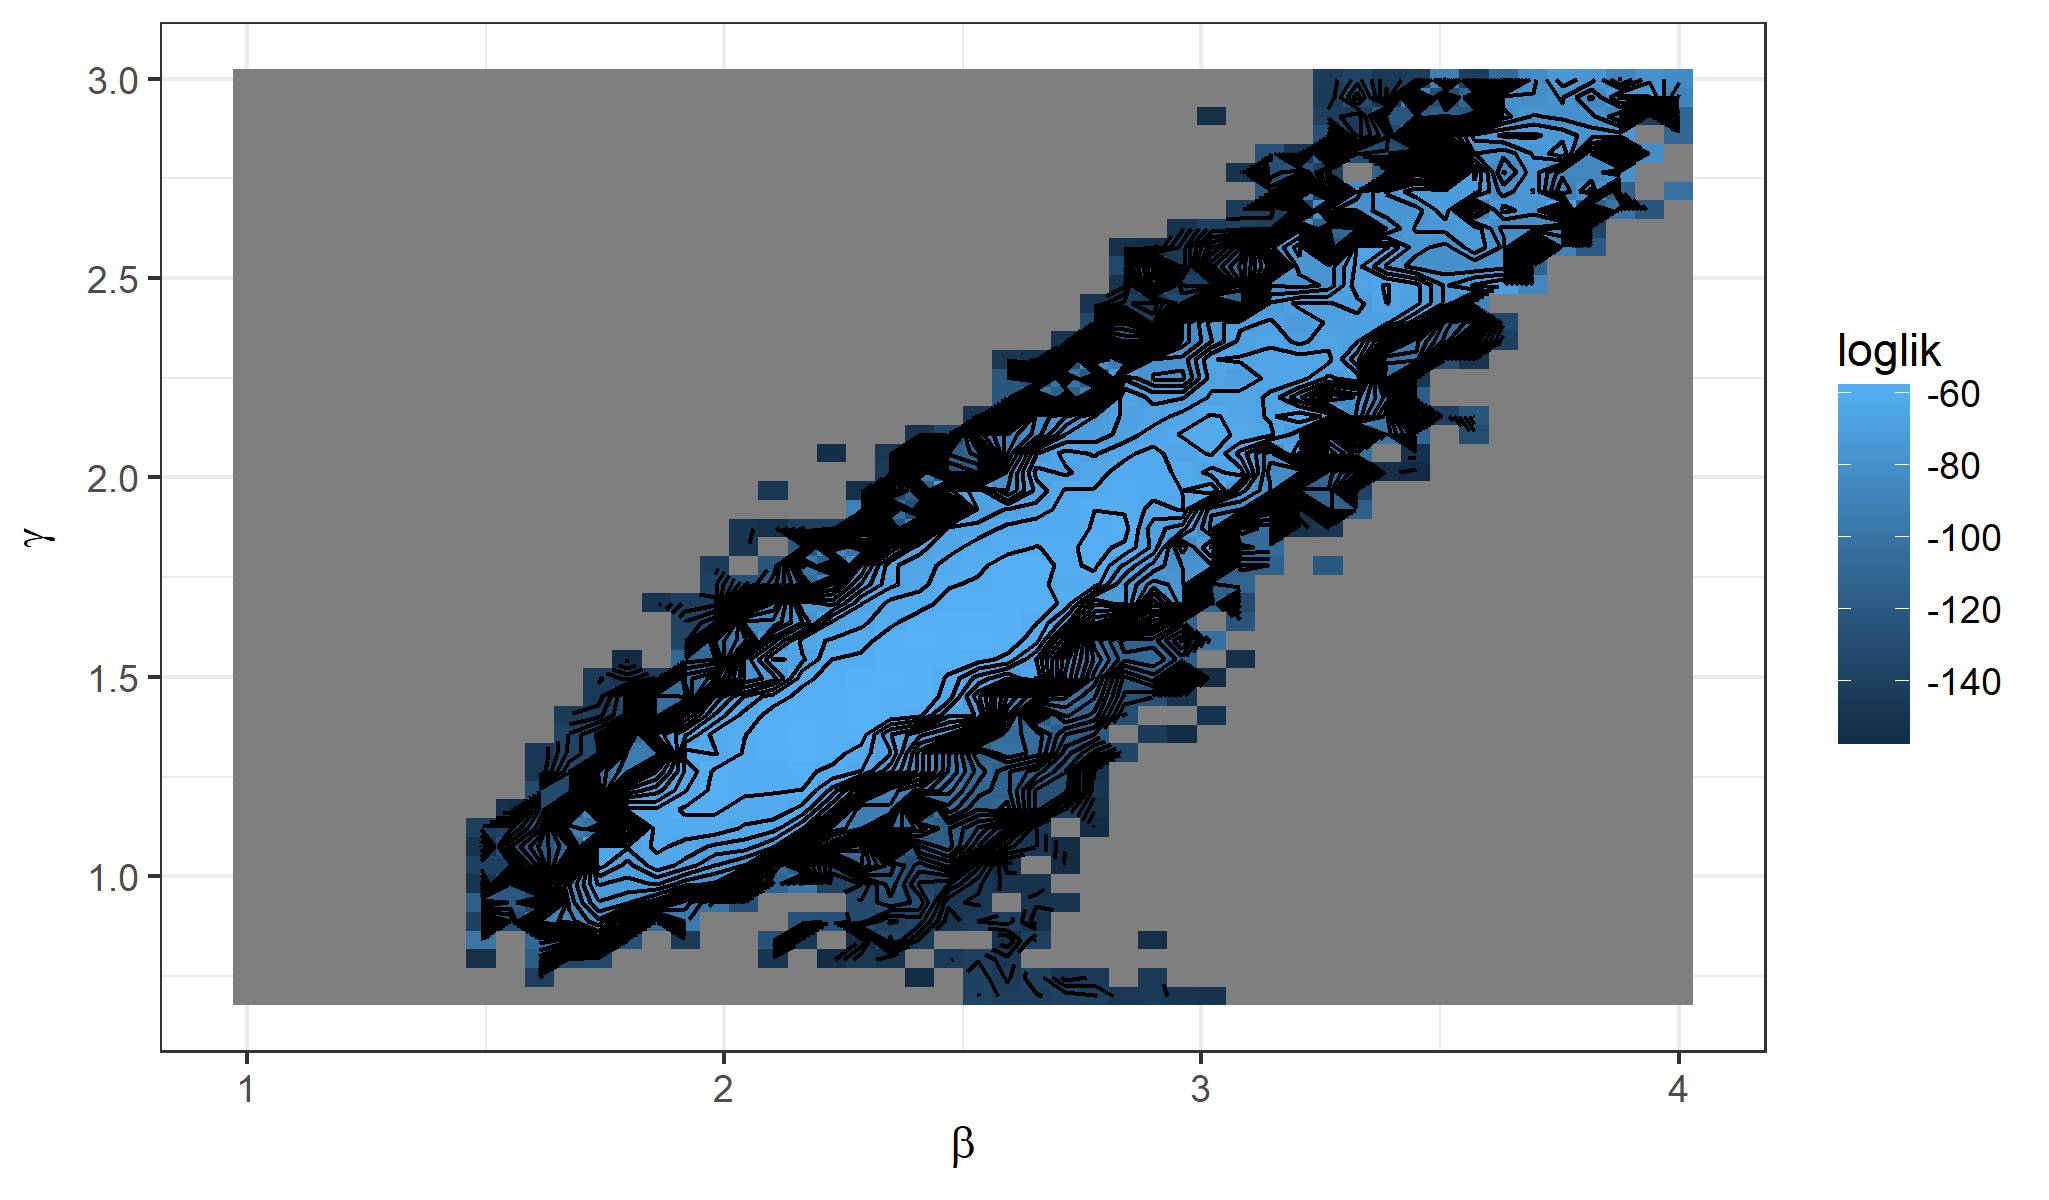
\includegraphics{figure/notes12-sir-grid1-plot-1} \end{center}

\begin{center}\rule{0.5\linewidth}{\linethickness}\end{center}

\subsubsection{Exercise: 2D likelihood
slice}\label{exercise-2d-likelihood-slice}

Compute a slice of the likelihood in the \(\beta\)-\(N\) plane.

\begin{center}\rule{0.5\linewidth}{\linethickness}\end{center}

\subsection{Maximizing the likelihood using the particle
filter}\label{maximizing-the-likelihood-using-the-particle-filter}

\begin{itemize}
\tightlist
\item
  First, a few cautionary words about parameter estimation for dynamic
  models
\end{itemize}

\subsubsection{Causal, mechanistic interpretation of parameter
estimates}\label{causal-mechanistic-interpretation-of-parameter-estimates}

\begin{itemize}
\item
  When we write down a mechanistic model for a system, we have some idea
  of what we intend parameters to mean. In epidemiology, for example, we
  interpret parameters as a reporting rate, a contact rate between
  individuals, an immigration rate, a duration of immunity, etc.
\item
  The data and the parameter estimation procedure do not know about our
  intended interpretation of the model. It can and does happen that some
  parameter estimates statistically consistent with the data may be
  scientifically absurd according to the scientific reasoning that went
  into building the model.
\item
  This can arise as a consequence of weak identifiability.
\item
  It can also be a warning that the data do not agree that our model
  represents reality in the way we had hoped. Perhaps more work is
  needed on model development.
\item
  Scientifically unreasonable parameter estimates can sometimes be
  avoided by fixing some parameters at known, reasonable values.
  However, this risks suppressing the warning that the data were trying
  to give about weaknesses in the model, or in the biological
  interpretation of it.
\item
  This issue will be discussed further when it arises in case studies.
\end{itemize}

\begin{center}\rule{0.5\linewidth}{\linethickness}\end{center}

\begin{center}\rule{0.5\linewidth}{\linethickness}\end{center}

\subsubsection{Likelihood maximization for the boarding school flu
example}\label{likelihood-maximization-for-the-boarding-school-flu-example}

\begin{itemize}
\item
  We saw above that the default parameter set for the `bsflu' pomp
  object is not particularly close to the MLE.
\item
  One way to find the MLE is to try optimizing the estimated likelihood,
  computed by the particle filter, directly.
\item
  There are many optimization algorithms to choose from, and many
  implemented in R.
\item
  Three issues arise immediately.
\end{itemize}

\begin{enumerate}
\def\labelenumi{\arabic{enumi}.}
\item
  The particle filter gives us a stochastic estimate of the likelihood.
  We can reduce this variability by making the number of particles,
  \texttt{Np}, larger. However, we cannot make it go away. If we use a
  deterministic optimizer (i.e., one that assumes the objective function
  is evaluated deterministically), then we must control this variability
  somehow. For example, we can fix the seed of the pseudo-random number
  generator. A side effect will be that the objective function becomes
  jagged, marked by many small local knolls and pits. Alternatively, we
  can use a stochastic optimization algorithm, with which we will be
  only be able to obtain estimates of our MLE. This is the trade-off
  between a noisy and a rough objective function.
\item
  Because the particle filter gives us just an estimate of the
  likelihood and no information about the derivative, we must choose an
  algorithm that is ``derivative-free''. There are many such, but we can
  expect less efficiency than would be possible with derivative
  information. Note that finite differencing is not an especially
  promising way of constructing derivatives. The price would be a
  \(n\)-fold increase in cpu time, where \(n\) is the dimension of the
  parameter space. Also, since the likelihood is only estimated, we
  would expect the derivative estimates to be noisy.
\item
  Finally, the parameters are constrained to be positive, and
  \(\rho < 1\). We must therefore select an optimizer that can solve
  this \emph{constrained maximization problem}, or figure out some of
  way of turning it into an unconstrained maximization problem. For the
  latter purpose, one can transform the parameters onto a scale on which
  there are no constraints.
\end{enumerate}

\begin{center}\rule{0.5\linewidth}{\linethickness}\end{center}

\begin{center}\rule{0.5\linewidth}{\linethickness}\end{center}

\subsection{An iterated filtering algorithm
(IF2)}\label{an-iterated-filtering-algorithm-if2}

\begin{itemize}
\item
  We use the IF2 algorithm of Ionides et al. (2015).
\item
  A particle filter is carried out with the parameter vector for each
  particle doing a random walk.
\item
  At the end of the time series, the collection of parameter vectors is
  recycled as starting parameters for a new particle filter with a
  smaller random walk variance.
\item
  Theoretically, this procedure converges toward the region of parameter
  space maximizing the maximum likelihood.
\item
  Empirically, we can test this claim on examples.
\end{itemize}

\subsubsection{IF2 algorithm pseudocode}\label{if2-algorithm-pseudocode}

\textbf{model input}: Simulators for \(f_{X_0}(x_0;\theta)\) and
\(f_{X_n|X_{n-1}}(x_n| x_{n-1}; \theta)\); evaluator for
\(f_{Y_n|X_n}(y_n| x_n;\theta)\); data, \(y^*_{1:N}\)

\textbf{algorithmic parameters}: Number of iterations, \(M\); number of
particles, \(J\); initial parameter swarm,
\(\{\Theta^0_j, j=1,\dots,J\}\); perturbation density,
\(h_n(\theta|\varphi;\sigma)\); perturbation scale, \(\sigma_{1{:}M}\)

\textbf{output}: Final parameter swarm, \(\{\Theta^M_j, j=1,\dots,J\}\)

\begin{enumerate}
\def\labelenumi{\arabic{enumi}.}
\tightlist
\item
  \(\quad\) For \(m\) in \(1{:} M\)
\item
  \(\quad\quad\quad\)
  \(\Theta^{F,m}_{0,j}\sim h_0(\theta|\Theta^{m-1}_{j}; \sigma_m)\) for
  \(j\) in \(1{:} J\)
\item
  \(\quad\quad\quad\)
  \(X_{0,j}^{F,m}\sim f_{X_0}(x_0 ; \Theta^{F,m}_{0,j})\) for \(j\) in
  \(1{:} J\)
\item
  \(\quad\quad\quad\) For \(n\) in \(1{:} N\)
\item
  \(\quad\quad\quad\quad\quad\)
  \(\Theta^{P,m}_{n,j}\sim h_n(\theta|\Theta^{F,m}_{n-1,j},\sigma_m)\)
  for \(j\) in \(1{:} J\)
\item
  \(\quad\quad\quad\quad\quad\)
  \(X_{n,j}^{P,m}\sim f_{X_n|X_{n-1}}(x_n | X^{F,m}_{n-1,j}; \Theta^{P,m}_j)\)
  for \(j\) in \(1{:} J\)
\item
  \(\quad\quad\quad\quad\quad\)
  \(w_{n,j}^m = f_{Y_n|X_n}(y^*_n| X_{n,j}^{P,m} ; \Theta^{P,m}_{n,j})\)
  for \(j\) in \(1{:} J\)
\item
  \(\quad\quad\quad\quad\quad\) Draw \(k_{1{:}J}\) with
  \(P[k_j=i]= w_{n,i}^m\Big/\sum_{u=1}^J w_{n,u}^m\)
\item
  \(\quad\quad\quad\quad\quad\)
  \(\Theta^{F,m}_{n,j}=\Theta^{P,m}_{n,k_j}\) and
  \(X^{F,m}_{n,j}=X^{P,m}_{n,k_j}\) for \(j\) in \(1{:} J\)
\item
  \(\quad\quad\quad\) End For
\item
  \(\quad\quad\quad\) Set \(\Theta^{m}_{j}=\Theta^{F,m}_{N,j}\) for
  \(j\) in \(1{:} J\)
\item
  \(\quad\) End For
\end{enumerate}

\textbf{comments}:

\begin{itemize}
\item
  The \(N\) loop (lines 4 through 10) is a basic particle filter applied
  to a model with stochastic perturbations to the parameters.
\item
  The \(M\) loop repeats this particle filter with decreasing
  perturbations.
\item
  The superscript \(F\) in \(\Theta^{F,m}_{n,j}\) and \(X^{F,m}_{n,j}\)
  denote solutions to the \emph{filtering} problem, with the particles
  \(j=1,\dots,J\) providing a Monte Carlo representation of the
  conditional distribution at time \(n\) given data \(y^*_{1:n}\) for
  filtering iteration \(m\).
\item
  The superscript \(P\) in \(\Theta^{P,m}_{n,j}\) and \(X^{P,m}_{n,j}\)
  denote solutions to the \emph{prediction} problem, with the particles
  \(j=1,\dots,J\) providing a Monte Carlo representation of the
  conditional distribution at time \(n\) given data \(y^*_{1:n-1}\) for
  filtering iteration \(m\).
\item
  The \emph{weight} \(w^m_{n,j}\) gives the likelihood of the data at
  time \(n\) for particle \(j\) in filtering iteration \(m\).
\end{itemize}

\subsubsection{Choosing the algorithmic settings for
IF2}\label{choosing-the-algorithmic-settings-for-if2}

\begin{itemize}
\item
  The initial parameter swarm, \(\{ \Theta^0_j, j=1,\dots,J\}\), usually
  consists of \(J\) identical replications of some starting parameter
  vector.
\item
  \(J\) is set to be sufficient for particle filtering. By the time of
  the last iteration (\(m=M\)) one should not have effective sample size
  close to 1.
\item
  Perturbations are usually chosen to be Gaussian, with \(\sigma_m\)
  being a scale factor for iteration \(m\):
  \[h_n(\theta|\varphi;\sigma) \sim N[\varphi, \sigma^2_m V_n].\]
\item
  \(V_n\) is usually taken to be diagonal,
  \[ V_n = \left( \begin{array}{ccccc}
  v_{1,n}^2 & 0 & 0 & \rightarrow & 0 \\
  0 & v_{2,n}^2 &  0 & \rightarrow & 0 \\
  0 & 0 & v_{3,n}^2 & \rightarrow & 0 \\
  \downarrow & & & \searrow & \downarrow \\
  0 & 0 & 0 & \rightarrow & v_{p,n}^2 \end{array}\right).\]
\item
  If \(\theta_i\) is a parameter that affects the dynamics or
  observations throughout the timeseries, it is called a \textbf{regular
  parameter}, and it is often appropriate to specify \[ v_{i,n} = v_i,\]
\item
  If \(\theta_j\) is a parameter that affects only the initial
  conditions of the dynamic model, it is called an \textbf{initial value
  parameter} (IVP) and it is appropriate to specify
  \[ v_{j,n} = \left\{\begin{array}{ll} v_j & \mbox{if $n=0$} \\
  0 & \mbox{if $n>0$} \end{array}\right.\]
\item
  If \(\theta_k\) is a break-point parameter that models how the system
  changes at time \(t_q\) then \(\theta_k\) is like an IVP at time
  \(t_q\) and it is appropriate to specify
  \[ v_{j,n} = \left\{\begin{array}{ll} v_j & \mbox{if $n=q$} \\
  0 & \mbox{if $n\neq q$} \end{array}\right.\]
\item
  \(\sigma_{1:M}\) is called a \textbf{cooling schedule}, following a
  thermodynamic analogy popularized by
  \href{https://en.wikipedia.org/wiki/Simulated_annealing}{simulated
  annealing}. As \(\sigma_m\) becomes small, the system cools toward a
  ``freezing point''. If the algorithm is working sucessfully, the
  freezing point should be close to the lowest-energy state of the
  system, i.e., the MLE.
\item
  It is generally helpful for optimization to provide transformations of
  the parameters so that (on the estimation scale) they are real-valued
  and have uncertainty on the order of 1 unit. For example, one
  typically takes a logarithmic transformation of positive parameters
  and a logistic transformation of \([0,1]\) valued parameters.
\item
  On this scale, it is surprisingly often effective to take
  \[ v_i = 0.02\] for regular parameters (RPs) and \[ v_j = 0.1\] for
  initial value parameters (IVPs).
\item
  We suppose that \(\sigma_1=1\), since the scale of the parameters is
  addressed by the matrix \(V_n\) . Early on in an investigation, one
  might take \(M=100\) and \(\sigma_M=0.1\). Later on, consideration of
  diagnostic plots may suggest refinements.
\item
  It is surprising that useful general advice exists for these
  quantities that could in principle be highly model-specific. Here is
  one possible explanation: the precision of interest is often the
  second significant figure and there are often order 100 observations
  (10 monthly obsevations would be too few to fit a mechanistic model;
  1000 would be unusual for an epidemiological system).
\end{itemize}

\begin{center}\rule{0.5\linewidth}{\linethickness}\end{center}

\begin{center}\rule{0.5\linewidth}{\linethickness}\end{center}

\subsection{Applying IF2 to a boarding school influenza
outbreak}\label{applying-if2-to-a-boarding-school-influenza-outbreak}

\begin{itemize}
\item
  We're going to reintroduce the boarding school flu example. This
  provides a reminder, but also lets us develop the model and the
  corresponding pomp object in a way that generalizes to other
  situations. It will be a template for the case studies that follow.
\item
  For a relatively simple epidemiological example of IF2, we consider
  fitting a stochastic SIR model to an influenza outbreak in a British
  boarding school (Anonymous 1978). Reports consist of the number of
  children confined to bed for each of the 14 days of the outbreak. The
  total number of children at the school was 763, and a total of 512
  children spent time away from class. Only one adult developed
  influenza-like illness, so adults are omitted from the data and model.
  First, we read in the boarding school flu (bsflu) data:
\end{itemize}

\begin{Shaded}
\begin{Highlighting}[]
\NormalTok{bsflu_data <-}\StringTok{ }\KeywordTok{read.table}\NormalTok{(}\StringTok{"bsflu_data.txt"}\NormalTok{)}
\end{Highlighting}
\end{Shaded}

\begin{itemize}
\item
  Our model is a variation on a basic SIR Markov chain, with state
  \(X(t)=(S(t),I(t),R_1(t),R_2(t),R_3(t) )\) giving the number of
  individuals in the susceptible and infectious categories, and three
  stages of recovery.
\item
  The recovery stages, \(R_1\), \(R_2\) and \(R_3\), are all modeled to
  be non-contagious.
\item
  \(R_1\) consists of individuals who are bed-confined if they show
  symptoms.
\item
  \(R_2\) consists of individuals who are convalescent if they showed
  symptoms.
\item
  \(R_3\) consists of recovered individuals who have returned to
  schoolwork if they were symtomatic.
\item
  The observation on day \(n\) of the observed epidemic (with \(n=1\)
  being 22 January) consists of the numbers of children who are
  bed-confined and convalescent.
\item
  These measurements are modeled as \(Y_n=(B_n,C_n)\) with
  \(B_n\sim\mathrm{Poisson}(\rho R_1(t_n))\) and
  \(C_n\sim\mathrm{Poisson}(\rho R_2(t_n))\).
\item
  Here, \(\rho\) is a reporting rate corresponding to the chance of
  being symptomatic.
\item
  The index case for the epidemic was proposed to be a boy returning to
  Britain from Hong Kong, who was reported to have a transient febrile
  illness from 15 to 18 January. It would therefore be reasonable to
  initialize the epidemic with \(I(t_0)=1\) at \(t_0=-6\). This is a
  little tricky to reconcile with the rest of the data; for now, we
  avoid this issue by instead initializing with \(I(t_0)=1\) at
  \(t_0=0\). All other individuals are modeled to be initially
  susceptible.
\item
  Our Markov transmission model is that each individual in \(S\)
  transitions to \(I\) at rate \(\beta I(t)\); each individual in \(I\)
  transitions at rate \(\mu_I\) to \(R_1\). Subsequently, the individual
  moves from \(R_1\) to \(R_2\) at rate \(\mu_{R_1}\), and finally from
  \(R_2\) to \(R_3\) at rate \(\mu_{R_2}\).
\item
  Therefore, \(1/\mu_I\) is the mean infectious time prior to
  bed-confinement; \(1/R_1\) is the mean duration of bed-confinement for
  symptomatic cases; \(1/R_2\) is the mean duration of convalescence for
  symptomatic cases. All rates have units \(\mathrm{day}^{-1}\).
\item
  This model has limitations and weaknesses. Writing down and fitting a
  model is a starting point for data analysis, not an end point. In
  particular, one should try model variations. For example, one could
  include a latency period for infections, or one could modify the model
  to give a better description of the bed-confinement and convalescence
  processes. Ten individuals received antibiotics for secondary
  infections, and they had longer bed-confinement and convalescence
  times. Partly for this reason, we will initially fit only the
  bed-confinement data, using \(Y_n=B_n\) for our \texttt{dmeasure}.
\item
  For the code, we represent the states (\(S\), \(I\), \(R_1\), \(R_2\))
  and the parameters (\(\beta\), \(\mu_I\), \(\rho\), \(\mu_{R_1}\),
  \(\mu_{R_2}\)) as follows:
\end{itemize}

\begin{Shaded}
\begin{Highlighting}[]
\NormalTok{bsflu_statenames <-}\StringTok{ }\KeywordTok{c}\NormalTok{(}\StringTok{"S"}\NormalTok{,}\StringTok{"I"}\NormalTok{,}\StringTok{"R1"}\NormalTok{,}\StringTok{"R2"}\NormalTok{)}
\NormalTok{bsflu_paramnames <-}\StringTok{ }\KeywordTok{c}\NormalTok{(}\StringTok{"Beta"}\NormalTok{,}\StringTok{"mu_I"}\NormalTok{,}\StringTok{"rho"}\NormalTok{,}\StringTok{"mu_R1"}\NormalTok{,}\StringTok{"mu_R2"}\NormalTok{)}
\end{Highlighting}
\end{Shaded}

The observation names (\(B\), \(C\)) are the names of the data
variables:

\begin{Shaded}
\begin{Highlighting}[]
\NormalTok{(bsflu_obsnames <-}\StringTok{ }\KeywordTok{colnames}\NormalTok{(bsflu_data)[}\DecValTok{1}\OperatorTok{:}\DecValTok{2}\NormalTok{])}
\end{Highlighting}
\end{Shaded}

\begin{verbatim}
## [1] "B" "C"
\end{verbatim}

We do not need a representation of \(R_3\) since the total population
size is fixed at \(P=763\) and hence
\(R_3(t)=P-S(t)-I(t)-R_1(t)-R_2(t)\). Now, we write the model code:

\begin{Shaded}
\begin{Highlighting}[]
\NormalTok{bsflu_dmeasure <-}\StringTok{ "}
\StringTok{  lik = dpois(B,rho*R1+1e-6,give_log);}
\StringTok{"}

\NormalTok{bsflu_rmeasure <-}\StringTok{ "}
\StringTok{  B = rpois(rho*R1+1e-6);}
\StringTok{  C = rpois(rho*R2);}
\StringTok{"}

\NormalTok{bsflu_rprocess <-}\StringTok{ "}
\StringTok{  double t1 = rbinom(S,1-exp(-Beta*I*dt));}
\StringTok{  double t2 = rbinom(I,1-exp(-dt*mu_I));}
\StringTok{  double t3 = rbinom(R1,1-exp(-dt*mu_R1));}
\StringTok{  double t4 = rbinom(R2,1-exp(-dt*mu_R2));}
\StringTok{  S -= t1;}
\StringTok{  I += t1 - t2;}
\StringTok{  R1 += t2 - t3;}
\StringTok{  R2 += t3 - t4;}
\StringTok{"}

\NormalTok{bsflu_fromEstimationScale <-}\StringTok{ "}
\StringTok{ TBeta = exp(Beta);}
\StringTok{ Tmu_I = exp(mu_I);}
\StringTok{ Trho = expit(rho);}
\StringTok{"}

\NormalTok{bsflu_toEstimationScale <-}\StringTok{ "}
\StringTok{ TBeta = log(Beta);}
\StringTok{ Tmu_I = log(mu_I);}
\StringTok{ Trho = logit(rho);}
\StringTok{"}

\NormalTok{bsflu_initializer <-}\StringTok{ "}
\StringTok{ S=762;}
\StringTok{ I=1;}
\StringTok{ R1=0;}
\StringTok{ R2=0;}
\StringTok{"}
\end{Highlighting}
\end{Shaded}

We can now build the new \texttt{bsflu} pomp object.

\begin{Shaded}
\begin{Highlighting}[]
\KeywordTok{require}\NormalTok{(pomp)}
\KeywordTok{stopifnot}\NormalTok{(}\KeywordTok{packageVersion}\NormalTok{(}\StringTok{"pomp"}\NormalTok{)}\OperatorTok{>=}\StringTok{"0.75-1"}\NormalTok{)}
\NormalTok{bsflu2 <-}\StringTok{ }\KeywordTok{pomp}\NormalTok{(}
  \DataTypeTok{data=}\NormalTok{bsflu_data,}
  \DataTypeTok{times=}\StringTok{"day"}\NormalTok{,}
  \DataTypeTok{t0=}\DecValTok{0}\NormalTok{,}
  \DataTypeTok{rprocess=}\KeywordTok{euler.sim}\NormalTok{(}
    \DataTypeTok{step.fun=}\KeywordTok{Csnippet}\NormalTok{(bsflu_rprocess),}
    \DataTypeTok{delta.t=}\DecValTok{1}\OperatorTok{/}\DecValTok{12}
\NormalTok{  ),}
  \DataTypeTok{rmeasure=}\KeywordTok{Csnippet}\NormalTok{(bsflu_rmeasure),}
  \DataTypeTok{dmeasure=}\KeywordTok{Csnippet}\NormalTok{(bsflu_dmeasure),}
  \DataTypeTok{fromEstimationScale=}\KeywordTok{Csnippet}\NormalTok{(bsflu_fromEstimationScale),}
  \DataTypeTok{toEstimationScale=}\KeywordTok{Csnippet}\NormalTok{(bsflu_toEstimationScale),}
  \DataTypeTok{obsnames =}\NormalTok{ bsflu_obsnames,}
  \DataTypeTok{statenames=}\NormalTok{bsflu_statenames,}
  \DataTypeTok{paramnames=}\NormalTok{bsflu_paramnames,}
  \DataTypeTok{initializer=}\KeywordTok{Csnippet}\NormalTok{(bsflu_initializer),}
  \DataTypeTok{cdir=}\KeywordTok{getwd}\NormalTok{()}
\NormalTok{)}
\KeywordTok{plot}\NormalTok{(bsflu2)}
\end{Highlighting}
\end{Shaded}

\begin{center}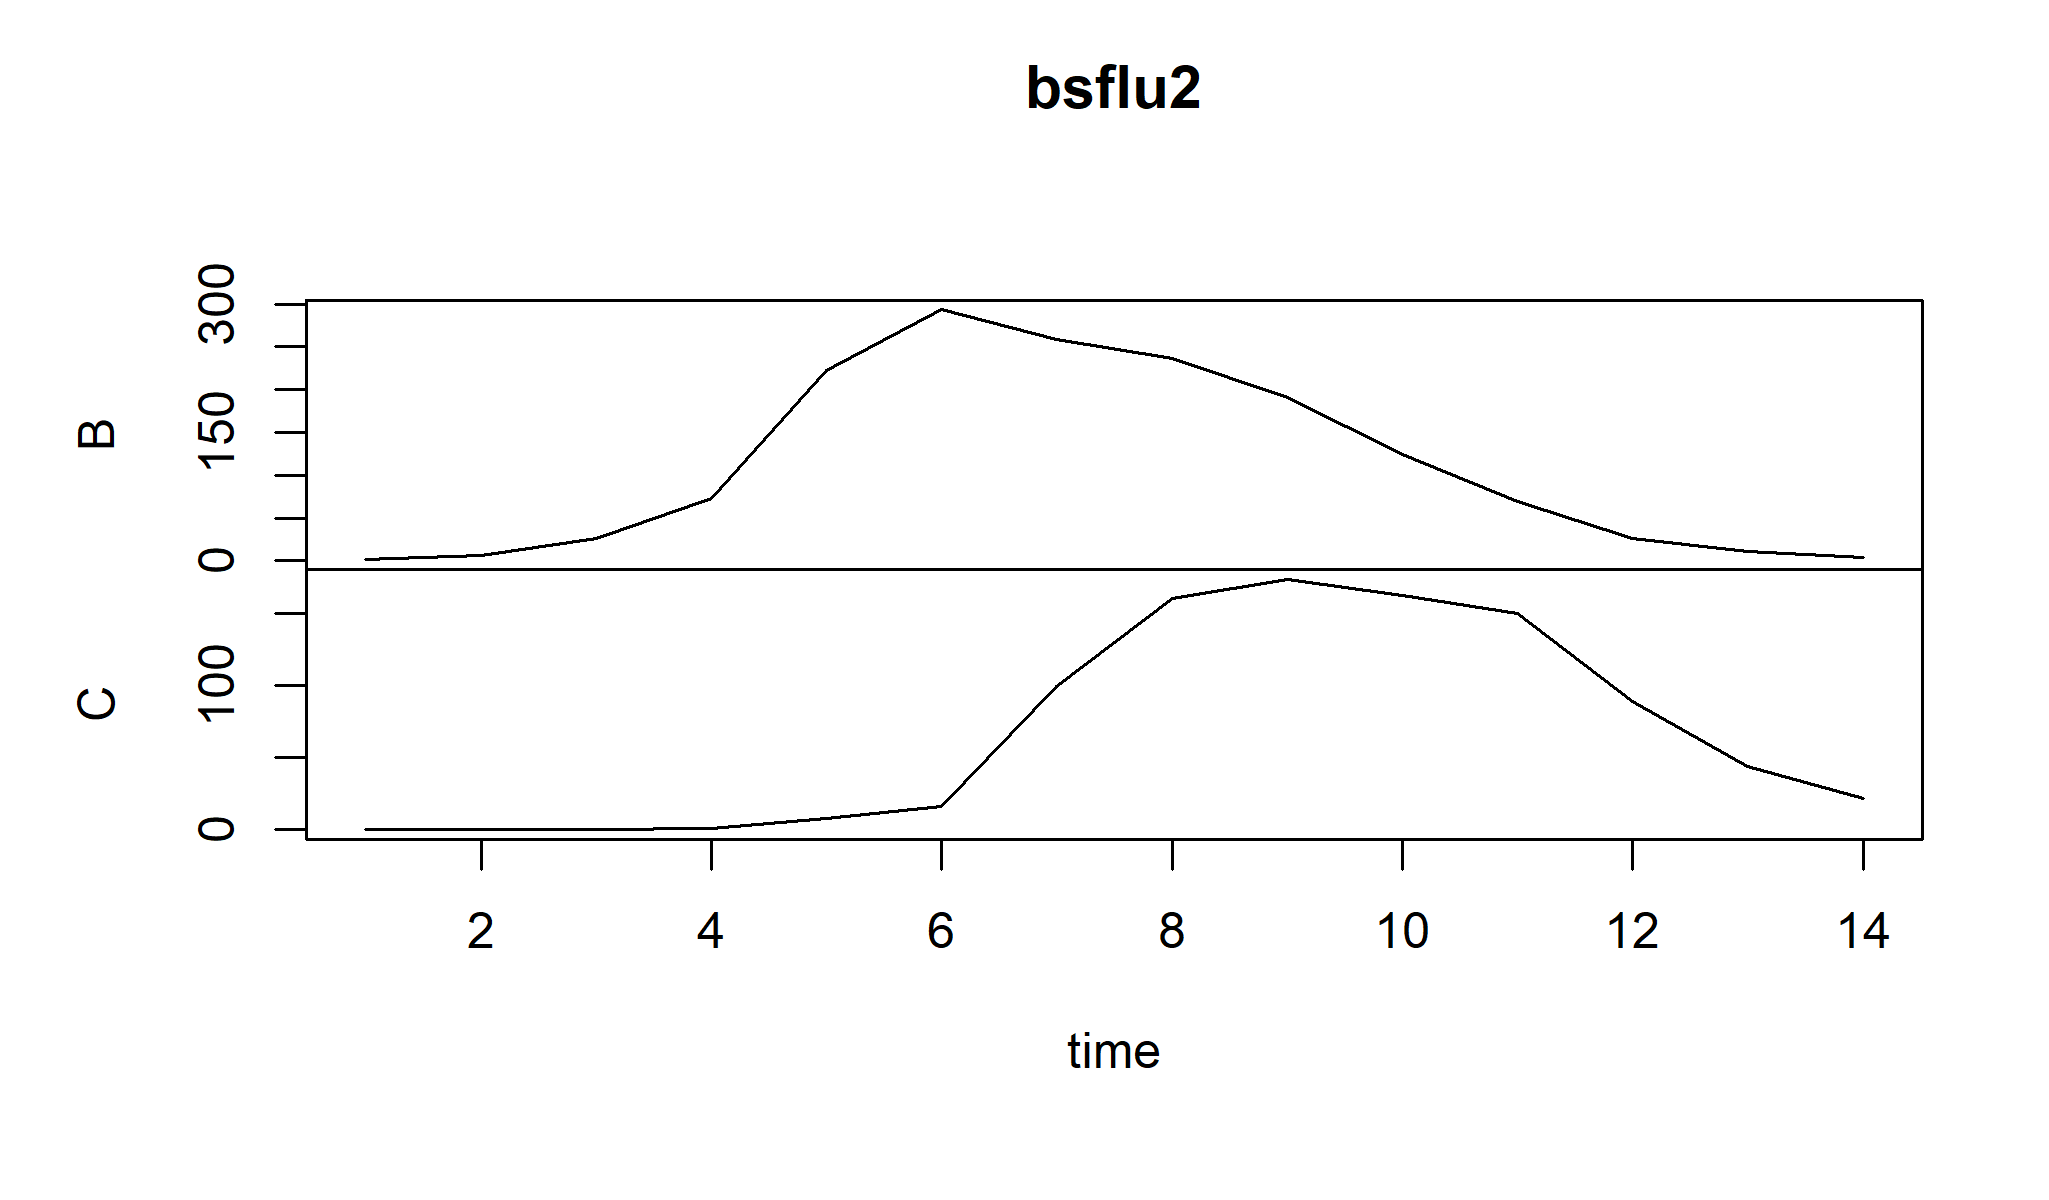
\includegraphics{figure/notes12-pomp_bsflu-1} \end{center}

\begin{itemize}
\tightlist
\item
  To develop and debug code, it is nice to have a version that runs
  extra quickly, for which we set \texttt{run\_level=1}. Here,
  \texttt{Np} is the number of particles (i.e., sequential Monte Carlo
  sample size), and \texttt{Nmif} is the number of iterations of the
  optimization procedure carried out below. Empirically,
  \texttt{Np=5000} and \texttt{Nmif=200} are around the minimum required
  to get stable results with an error in the likelihood of order 1 log
  unit for this example; this is implemented by setting
  \texttt{run\_level=2}. One can then ramp up to larger values for more
  refined computations, implemented here by \texttt{run\_level=3}.
\end{itemize}

\begin{Shaded}
\begin{Highlighting}[]
\NormalTok{run_level <-}\StringTok{ }\DecValTok{3}
\ControlFlowTok{switch}\NormalTok{(run_level,}
\NormalTok{       \{bsflu_Np=}\DecValTok{100}\NormalTok{; bsflu_Nmif=}\DecValTok{10}\NormalTok{; bsflu_Neval=}\DecValTok{10}\NormalTok{; bsflu_Nglobal=}\DecValTok{10}\NormalTok{; bsflu_Nlocal=}\DecValTok{10}\NormalTok{\}, }
\NormalTok{       \{bsflu_Np=}\DecValTok{20000}\NormalTok{; bsflu_Nmif=}\DecValTok{100}\NormalTok{; bsflu_Neval=}\DecValTok{10}\NormalTok{; bsflu_Nglobal=}\DecValTok{10}\NormalTok{; bsflu_Nlocal=}\DecValTok{10}\NormalTok{\}, }
\NormalTok{       \{bsflu_Np=}\DecValTok{60000}\NormalTok{; bsflu_Nmif=}\DecValTok{300}\NormalTok{; bsflu_Neval=}\DecValTok{10}\NormalTok{; bsflu_Nglobal=}\DecValTok{100}\NormalTok{; bsflu_Nlocal=}\DecValTok{20}\NormalTok{\}}
\NormalTok{)}
\end{Highlighting}
\end{Shaded}

\subsubsection{Running a particle
filter}\label{running-a-particle-filter}

Before engaging in iterated filtering, it is often a good idea to check
that the basic particle filter is working since iterated filtering
builds on this technique. Here, carrying out slightly circular
reasoning, we are going to test \texttt{pfilter} on a previously
computed point estimate read in from \url{bsflu_params.csv}:

\begin{Shaded}
\begin{Highlighting}[]
\NormalTok{bsflu_params <-}\StringTok{ }\KeywordTok{data.matrix}\NormalTok{(}\KeywordTok{read.table}\NormalTok{(}\StringTok{"mif_bsflu_params.csv"}\NormalTok{,}\DataTypeTok{row.names=}\OtherTok{NULL}\NormalTok{,}\DataTypeTok{header=}\OtherTok{TRUE}\NormalTok{))}
\NormalTok{bsflu_mle <-}\StringTok{ }\NormalTok{bsflu_params[}\KeywordTok{which.max}\NormalTok{(bsflu_params[,}\StringTok{"logLik"}\NormalTok{]),][bsflu_paramnames]}
\end{Highlighting}
\end{Shaded}

We are going to treat \(\mu_{R_1}\) and \(\mu_{R_2}\) as known, fixed at
the empirical mean of the bed-confinement and convalescence times for
symptomatic cases:

\begin{Shaded}
\begin{Highlighting}[]
\NormalTok{bsflu_fixed_params <-}\StringTok{ }\KeywordTok{c}\NormalTok{(}\DataTypeTok{mu_R1=}\DecValTok{1}\OperatorTok{/}\NormalTok{(}\KeywordTok{sum}\NormalTok{(bsflu_data}\OperatorTok{$}\NormalTok{B)}\OperatorTok{/}\DecValTok{512}\NormalTok{),}\DataTypeTok{mu_R2=}\DecValTok{1}\OperatorTok{/}\NormalTok{(}\KeywordTok{sum}\NormalTok{(bsflu_data}\OperatorTok{$}\NormalTok{C)}\OperatorTok{/}\DecValTok{512}\NormalTok{))}
\end{Highlighting}
\end{Shaded}

\begin{itemize}
\item
  It is convenient to do some parallelization to speed up the
  computations. Most machines are multi-core nowadays, and using this
  computational capacity involves only

  \begin{enumerate}
  \def\labelenumi{\arabic{enumi}.}
  \item
    the following lines of code to let R know you plan to use multiple
    processors;
  \item
    using the parallel for loop provided by `foreach'.
  \end{enumerate}
\end{itemize}

\begin{Shaded}
\begin{Highlighting}[]
\KeywordTok{require}\NormalTok{(doParallel)}
\NormalTok{cores <-}\StringTok{ }\DecValTok{20}  \CommentTok{# The number of cores on this machine }
\KeywordTok{registerDoParallel}\NormalTok{(cores)}
\NormalTok{mcopts <-}\StringTok{ }\KeywordTok{list}\NormalTok{(}\DataTypeTok{set.seed=}\OtherTok{TRUE}\NormalTok{)}

\KeywordTok{set.seed}\NormalTok{(}\DecValTok{396658101}\NormalTok{,}\DataTypeTok{kind=}\StringTok{"L'Ecuyer"}\NormalTok{)}
\end{Highlighting}
\end{Shaded}

\begin{itemize}
\tightlist
\item
  Note that this code uses the \texttt{doParallel} library, whereas
  before we used \texttt{doMC}, as below.
\end{itemize}

\begin{Shaded}
\begin{Highlighting}[]
\KeywordTok{require}\NormalTok{(doMC)}
\KeywordTok{registerDoMC}\NormalTok{(}\DataTypeTok{cores=}\DecValTok{20}\NormalTok{) }
\end{Highlighting}
\end{Shaded}

\begin{itemize}
\item
  \texttt{doParallel} and \texttt{doMC} are functionally equivalent for
  our current purposes, but give you two options if you hit technical
  problems accessing the multiple cores on your machine.
\item
  We proceed to carry out replicated particle filters at this tentative
  MLE:
\end{itemize}

\begin{Shaded}
\begin{Highlighting}[]
\KeywordTok{stew}\NormalTok{(}\DataTypeTok{file=}\KeywordTok{sprintf}\NormalTok{(}\StringTok{"pf-%d.rda"}\NormalTok{,run_level),\{}
\NormalTok{  t_pf <-}\StringTok{ }\KeywordTok{system.time}\NormalTok{(}
\NormalTok{    pf <-}\StringTok{ }\KeywordTok{foreach}\NormalTok{(}\DataTypeTok{i=}\DecValTok{1}\OperatorTok{:}\DecValTok{20}\NormalTok{,}\DataTypeTok{.packages=}\StringTok{'pomp'}\NormalTok{,}
                  \DataTypeTok{.options.multicore=}\NormalTok{mcopts) }\OperatorTok\StringTok{ }\KeywordTok{try}\NormalTok{(}
                    \KeywordTok{pfilter}\NormalTok{(bsflu2,}\DataTypeTok{params=}\NormalTok{bsflu_mle,}\DataTypeTok{Np=}\NormalTok{bsflu_Np)}
\NormalTok{                  )}
\NormalTok{  )}
  
\NormalTok{\},}\DataTypeTok{seed=}\DecValTok{1320290398}\NormalTok{,}\DataTypeTok{kind=}\StringTok{"L'Ecuyer"}\NormalTok{)}

\NormalTok{(L_pf <-}\StringTok{ }\KeywordTok{logmeanexp}\NormalTok{(}\KeywordTok{sapply}\NormalTok{(pf,logLik),}\DataTypeTok{se=}\OtherTok{TRUE}\NormalTok{))}
\end{Highlighting}
\end{Shaded}

\begin{verbatim}
##                      se 
## -73.3241678   0.3197182
\end{verbatim}

\begin{itemize}
\tightlist
\item
  In 9.4 seconds, we obtain an unbiased likelihood estimate of -73.32
  with a Monte standard error of 0.32.
\end{itemize}

\subsubsection{Caching computations in
Rmarkdown}\label{caching-computations-in-rmarkdown}

\begin{itemize}
\item
  It is not unusual for computations in a POMP analysis to take hours to
  run on many cores.
\item
  The computations for a final version of a manuscript may take days.
\item
  Usually, we use some mechanism like the different values of
  \texttt{run\_level} so that preliminary versions of the manuscript
  take less time to run.
\item
  However, when editing the text or working on a different part of the
  manuscript, we don't want to re-run long pieces of code.
\item
  Saving results so that the code is only re-run when necessary is
  called \textbf{caching}.
\item
  You may already be familiar with Rmarkdown's own version of caching.
\item
  In the notes, we tell Rmarkdown to cache. For example, in
  (notes13.Rmd) the first R chunk, called \texttt{knitr-opts}, contains
  the following:
\end{itemize}

\begin{Shaded}
\begin{Highlighting}[]
\NormalTok{opts_chunk}\OperatorTok{$}\KeywordTok{set}\NormalTok{(}
  \DataTypeTok{cache=}\OtherTok{TRUE}\NormalTok{,}
\NormalTok{  )}
\end{Highlighting}
\end{Shaded}

\begin{itemize}
\item
  Rmarkdown uses a library called \texttt{knitr} to process the Rmd
  file, so options for Rmarkdown are formally options for knitr.
\item
  Having set the option \texttt{cache=TRUE}, Rmarkdown caches every
  chunk, meaning that a chunk will only be re-run if code in that chunk
  is edited.
\item
  You can force Rmarkdown to recompute all the chunks by deleting the
  \texttt{cache} subdirectory.
\item
  What if changes elsewhere in the document affect the proper evaluation
  of your chunk, but you didn't edit any of the code in the chunk
  itself?

  \begin{itemize}
  \tightlist
  \item
    Rmarkdown will get this wrong. \textbf{It will not recompute the
    chunk}.
  \end{itemize}
\item
  A perfect caching system doesn't exist. \textbf{Always delete the
  entire cache and rebuild a fresh cache before finishing a manuscript.}
\item
  Rmarkdown caching is good for relatively small computations, such as
  producing figures or things that may take a minute or two and are
  annoying if you have to recompute them every time you make any edits
  to the text.
\item
  For longer computations, it is good to have full manual control. In
  \textbf{pomp}, this is provided by two related functions,
  \texttt{stew} and \texttt{bake}.
\end{itemize}

\paragraph{\texorpdfstring{\texttt{stew} and
\texttt{bake}}{stew and bake}}\label{stew-and-bake}

\begin{itemize}
\item
  Notice the function \texttt{stew} in the replicated particle filter
  code above.
\item
  Here, \texttt{stew} looks for a file called
  \texttt{pf-{[}run\_level{]}.rda}.
\item
  If it finds this file, it simply loads the contents of this file.
\item
  If the file doesn't exist, it carries out the specified computation
  and saves it in a file of this name.
\item
  \texttt{bake} is similar to
  \texttt{stew.\ The\ difference\ is\ that}bake\texttt{uses}readRDS\texttt{and}saveRDS\texttt{,\ whereas}stew\texttt{uses}load\texttt{and}save`.
\item
  either way, the computation will not be re-run unless you manually
  delete \texttt{pf-{[}run\_level{]}.rda}.
\item
  \texttt{stew} and \texttt{bake} reset the seed appropriately whether
  or not the computation is recomputed. Othewise, caching risks adverse
  consequences for reproducibility.
\end{itemize}

\begin{center}\rule{0.5\linewidth}{\linethickness}\end{center}

\begin{center}\rule{0.5\linewidth}{\linethickness}\end{center}

\subsection{A local search of the likelihood
surface}\label{a-local-search-of-the-likelihood-surface}

\begin{itemize}
\tightlist
\item
  Let's carry out a local search using \texttt{mif2} around this
  previously identified MLE. For that, we need to set the \texttt{rw.sd}
  and \texttt{cooling.fraction.50} algorithmic parameters:
\end{itemize}

\begin{Shaded}
\begin{Highlighting}[]
\NormalTok{bsflu_rw.sd <-}\StringTok{ }\FloatTok{0.02}
\NormalTok{bsflu_cooling.fraction.}\DecValTok{50}\NormalTok{ <-}\StringTok{ }\FloatTok{0.5}

\KeywordTok{stew}\NormalTok{(}\DataTypeTok{file=}\KeywordTok{sprintf}\NormalTok{(}\StringTok{"local_search-%d.rda"}\NormalTok{,run_level),\{}
  
\NormalTok{  t_local <-}\StringTok{ }\KeywordTok{system.time}\NormalTok{(\{}
\NormalTok{    mifs_local <-}\StringTok{ }\KeywordTok{foreach}\NormalTok{(}\DataTypeTok{i=}\DecValTok{1}\OperatorTok{:}\NormalTok{bsflu_Nlocal,}\DataTypeTok{.packages=}\StringTok{'pomp'}\NormalTok{, }\DataTypeTok{.combine=}\NormalTok{c, }\DataTypeTok{.options.multicore=}\NormalTok{mcopts) }\OperatorTok\StringTok{  }\NormalTok{\{}
      \KeywordTok{mif2}\NormalTok{(}
\NormalTok{        bsflu2,}
        \DataTypeTok{start=}\NormalTok{bsflu_mle,}
        \DataTypeTok{Np=}\NormalTok{bsflu_Np,}
        \DataTypeTok{Nmif=}\NormalTok{bsflu_Nmif,}
        \DataTypeTok{cooling.type=}\StringTok{"geometric"}\NormalTok{,}
        \DataTypeTok{cooling.fraction.50=}\NormalTok{bsflu_cooling.fraction.}\DecValTok{50}\NormalTok{,}
        \DataTypeTok{transform=}\OtherTok{TRUE}\NormalTok{,}
        \DataTypeTok{rw.sd=}\KeywordTok{rw.sd}\NormalTok{(}
          \DataTypeTok{Beta=}\NormalTok{bsflu_rw.sd,}
          \DataTypeTok{mu_I=}\NormalTok{bsflu_rw.sd,}
          \DataTypeTok{rho=}\NormalTok{bsflu_rw.sd}
\NormalTok{        )}
\NormalTok{      )}
      
\NormalTok{    \}}
\NormalTok{  \})}
  
\NormalTok{\},}\DataTypeTok{seed=}\DecValTok{900242057}\NormalTok{,}\DataTypeTok{kind=}\StringTok{"L'Ecuyer"}\NormalTok{)}
\end{Highlighting}
\end{Shaded}

\begin{itemize}
\item
  Although the filtering carried out by \texttt{mif2} in the final
  filtering iteration generates an approximation to the likelihood at
  the resulting point estimate, this is not usually good enough for
  reliable inference. Partly, this is because some parameter
  perturbations remain in the last filtering iteration. Partly, this is
  because \texttt{mif2} is usually carried out with a smaller number of
  particles than is necessary for a good likelihood evaluation---the
  errors in \texttt{mif2} average out over many iterations of the
  filtering.
\item
  Therefore, we evaluate the likelihood, together with a standard error,
  using replicated particle filters at each point estimate:
\end{itemize}

\begin{Shaded}
\begin{Highlighting}[]
\KeywordTok{stew}\NormalTok{(}\DataTypeTok{file=}\KeywordTok{sprintf}\NormalTok{(}\StringTok{"lik_local-%d.rda"}\NormalTok{,run_level),\{}
\NormalTok{    t_local_eval <-}\StringTok{ }\KeywordTok{system.time}\NormalTok{(\{}
\NormalTok{    liks_local <-}\StringTok{ }\KeywordTok{foreach}\NormalTok{(}\DataTypeTok{i=}\DecValTok{1}\OperatorTok{:}\NormalTok{bsflu_Nlocal,}\DataTypeTok{.packages=}\StringTok{'pomp'}\NormalTok{,}\DataTypeTok{.combine=}\NormalTok{rbind) }\OperatorTok\StringTok{ }\NormalTok{\{}
\NormalTok{      evals <-}\StringTok{ }\KeywordTok{replicate}\NormalTok{(bsflu_Neval, }\KeywordTok{logLik}\NormalTok{(}\KeywordTok{pfilter}\NormalTok{(bsflu2,}\DataTypeTok{params=}\KeywordTok{coef}\NormalTok{(mifs_local[[i]]),}\DataTypeTok{Np=}\NormalTok{bsflu_Np)))}
      \KeywordTok{logmeanexp}\NormalTok{(evals, }\DataTypeTok{se=}\OtherTok{TRUE}\NormalTok{)}
\NormalTok{    \}}
\NormalTok{  \})}
\NormalTok{\},}\DataTypeTok{seed=}\DecValTok{900242057}\NormalTok{,}\DataTypeTok{kind=}\StringTok{"L'Ecuyer"}\NormalTok{)}

\NormalTok{results_local <-}\StringTok{ }\KeywordTok{data.frame}\NormalTok{(}\DataTypeTok{logLik=}\NormalTok{liks_local[,}\DecValTok{1}\NormalTok{],}\DataTypeTok{logLik_se=}\NormalTok{liks_local[,}\DecValTok{2}\NormalTok{],}\KeywordTok{t}\NormalTok{(}\KeywordTok{sapply}\NormalTok{(mifs_local,coef)))}
\KeywordTok{summary}\NormalTok{(results_local}\OperatorTok{$}\NormalTok{logLik,}\DataTypeTok{digits=}\DecValTok{5}\NormalTok{)}
\end{Highlighting}
\end{Shaded}

\begin{verbatim}
##    Min. 1st Qu.  Median    Mean 3rd Qu.    Max. 
##  -74.54  -74.24  -74.04  -74.01  -73.93  -73.30
\end{verbatim}

\begin{itemize}
\tightlist
\item
  This investigation took 48.1 minutes for the maximization and 1.5
  minutes for the likelihood evaluation. These repeated stochastic
  maximizations can also show us the geometry of the likelihood surface
  in a neighborhood of this point estimate:
\end{itemize}

\begin{Shaded}
\begin{Highlighting}[]
\KeywordTok{pairs}\NormalTok{(}\OperatorTok{~}\NormalTok{logLik}\OperatorTok{+}\NormalTok{Beta}\OperatorTok{+}\NormalTok{mu_I}\OperatorTok{+}\NormalTok{rho,}\DataTypeTok{data=}\KeywordTok{subset}\NormalTok{(results_local,logLik}\OperatorTok{>}\KeywordTok{max}\NormalTok{(logLik)}\OperatorTok{-}\DecValTok{50}\NormalTok{))}
\end{Highlighting}
\end{Shaded}

\begin{center}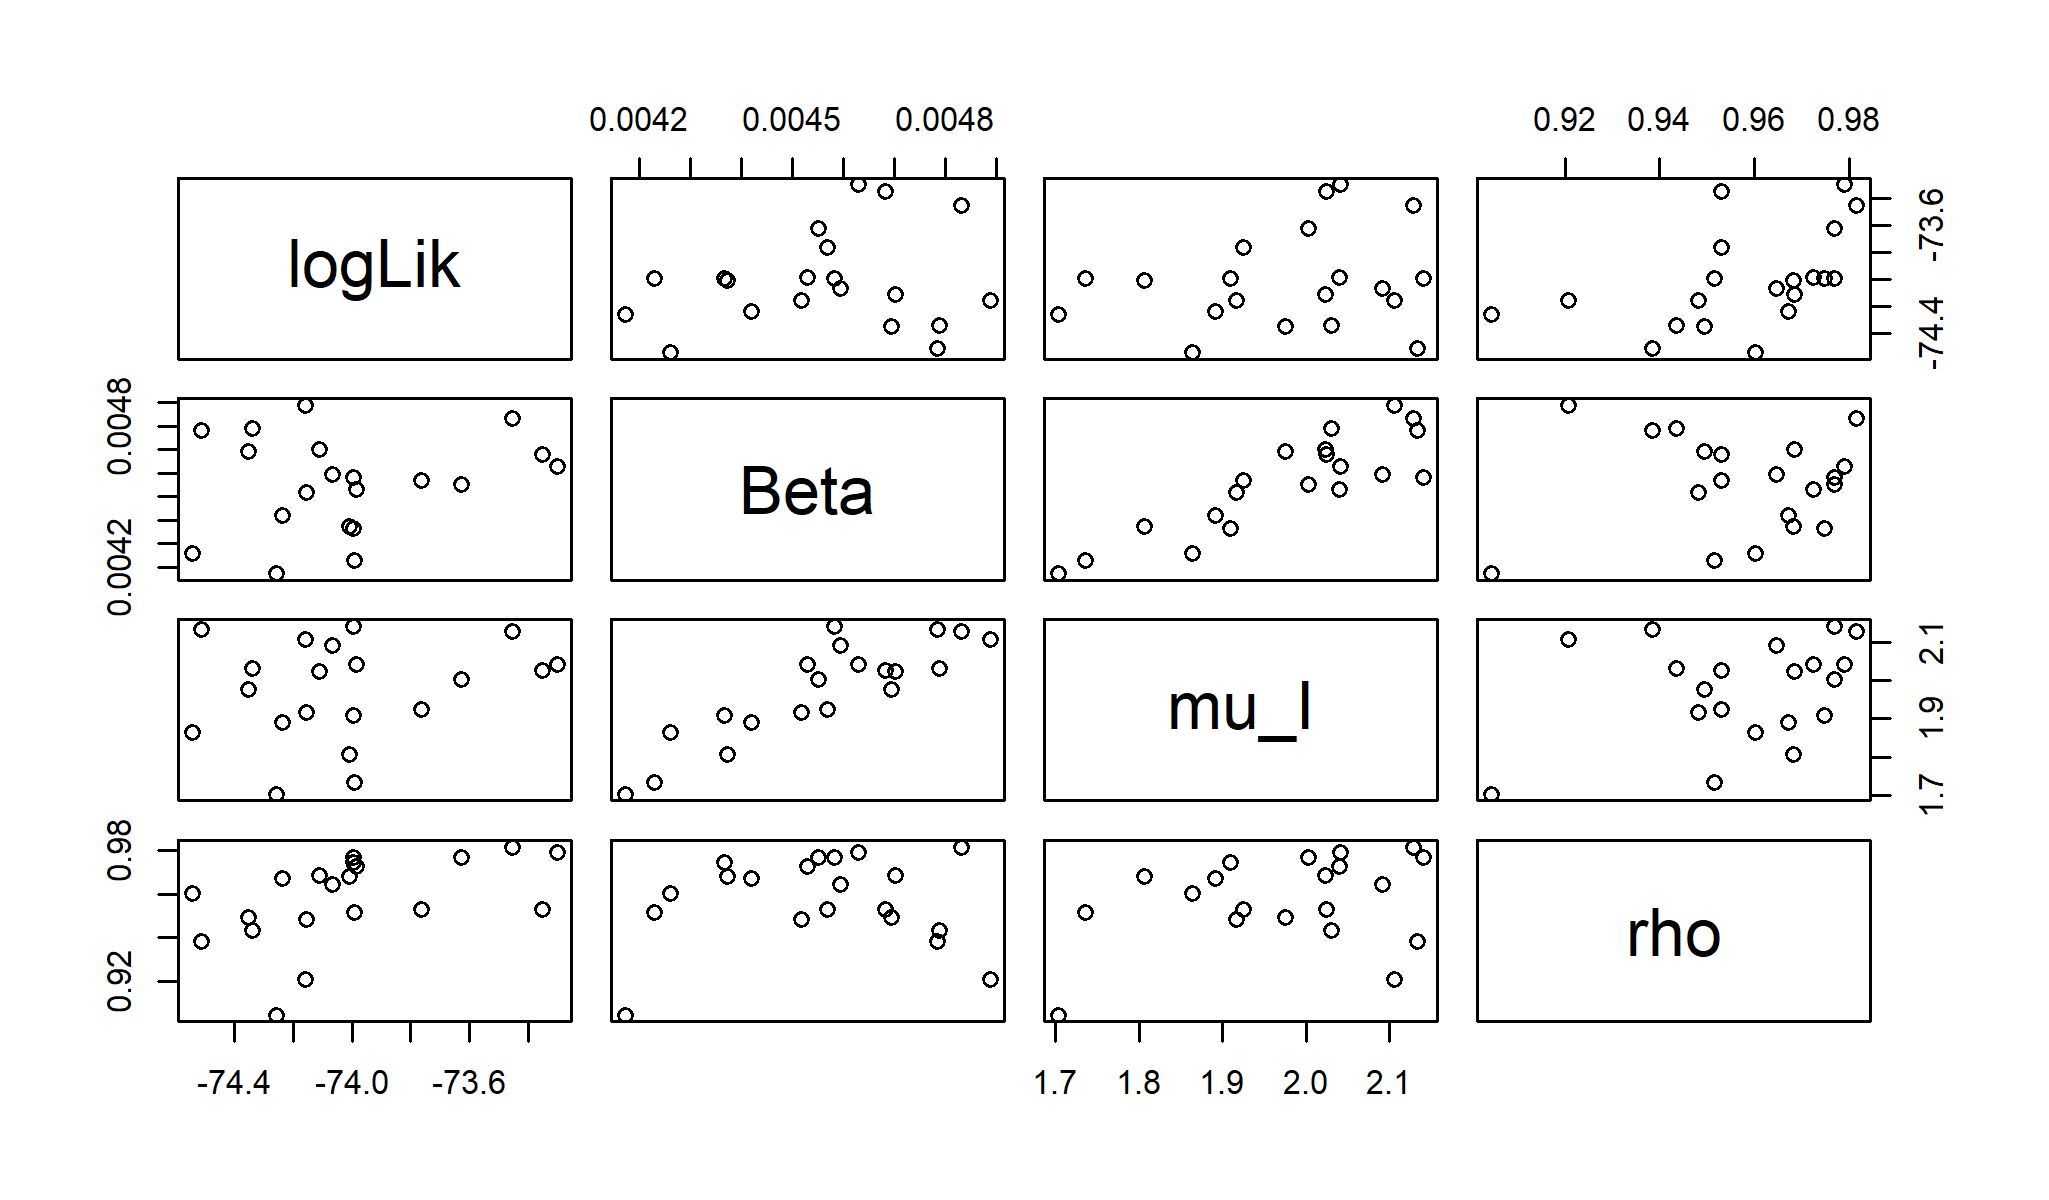
\includegraphics{figure/notes12-pairs_local-1} \end{center}

\begin{center}\rule{0.5\linewidth}{\linethickness}\end{center}

\begin{center}\rule{0.5\linewidth}{\linethickness}\end{center}

\subsection{A global search of the likelihood surface using randomized
starting
values}\label{a-global-search-of-the-likelihood-surface-using-randomized-starting-values}

\begin{itemize}
\item
  When carrying out parameter estimation for dynamic systems, we need to
  specify beginning values for both the dynamic system (in the state
  space) and the parameters (in the parameter space). By convention, we
  use \emph{initial values} for the initialization of the dynamic system
  and \emph{starting values} for initialization of the parameter search.
\item
  Practical parameter estimation involves trying many starting values
  for the parameters. One can specify a large box in parameter space
  that contains all parameter vectors which seem remotely sensible. If
  an estimation method gives stable conclusions with starting values
  drawn randomly from this box, this gives some confidence that an
  adequate global search has been carried out.
\item
  For our flu model, a box containing reasonable parameter values might
  be
\end{itemize}

\begin{Shaded}
\begin{Highlighting}[]
\NormalTok{bsflu_box <-}\StringTok{ }\KeywordTok{rbind}\NormalTok{(}
  \DataTypeTok{Beta=}\KeywordTok{c}\NormalTok{(}\FloatTok{0.001}\NormalTok{,}\FloatTok{0.01}\NormalTok{),}
  \DataTypeTok{mu_I=}\KeywordTok{c}\NormalTok{(}\FloatTok{0.5}\NormalTok{,}\DecValTok{2}\NormalTok{),}
  \DataTypeTok{rho =} \KeywordTok{c}\NormalTok{(}\FloatTok{0.5}\NormalTok{,}\DecValTok{1}\NormalTok{)}
\NormalTok{)}
\end{Highlighting}
\end{Shaded}

\begin{itemize}
\tightlist
\item
  We are now ready to carry out likelihood maximizations from diverse
  starting points. To simplify the code, we can reset only the starting
  parameters from \texttt{mifs\_global{[}{[}1{]}{]}} since the rest of
  the call to \texttt{mif2} can be read in from
  \texttt{mifs\_global{[}{[}1{]}{]}}:
\end{itemize}

\begin{Shaded}
\begin{Highlighting}[]
\KeywordTok{stew}\NormalTok{(}\DataTypeTok{file=}\KeywordTok{sprintf}\NormalTok{(}\StringTok{"box_eval-%d.rda"}\NormalTok{,run_level),\{}
  
\NormalTok{  t_global <-}\StringTok{ }\KeywordTok{system.time}\NormalTok{(\{}
\NormalTok{    mifs_global <-}\StringTok{ }\KeywordTok{foreach}\NormalTok{(}\DataTypeTok{i=}\DecValTok{1}\OperatorTok{:}\NormalTok{bsflu_Nglobal,}\DataTypeTok{.packages=}\StringTok{'pomp'}\NormalTok{, }\DataTypeTok{.combine=}\NormalTok{c, }\DataTypeTok{.options.multicore=}\NormalTok{mcopts) }\OperatorTok\StringTok{  }\KeywordTok{mif2}\NormalTok{(}
\NormalTok{      mifs_local[[}\DecValTok{1}\NormalTok{]],}
      \DataTypeTok{start=}\KeywordTok{c}\NormalTok{(}\KeywordTok{apply}\NormalTok{(bsflu_box,}\DecValTok{1}\NormalTok{,}\ControlFlowTok{function}\NormalTok{(x)}\KeywordTok{runif}\NormalTok{(}\DecValTok{1}\NormalTok{,x[}\DecValTok{1}\NormalTok{],x[}\DecValTok{2}\NormalTok{])),bsflu_fixed_params)}
\NormalTok{    )}
\NormalTok{  \})}
\NormalTok{\},}\DataTypeTok{seed=}\DecValTok{1270401374}\NormalTok{,}\DataTypeTok{kind=}\StringTok{"L'Ecuyer"}\NormalTok{)}
\end{Highlighting}
\end{Shaded}

\begin{itemize}
\tightlist
\item
  As noted above, the approximate likelihood evaluation generated by
  \texttt{mif2} in the final filtering iteration is not usually good
  enough for reliable inference. Therefore, we evaluate the likelihood,
  together with a standard error, using replicated particle filters at
  each point estimate:
\end{itemize}

\begin{Shaded}
\begin{Highlighting}[]
\KeywordTok{stew}\NormalTok{(}\DataTypeTok{file=}\KeywordTok{sprintf}\NormalTok{(}\StringTok{"lik_global_eval-%d.rda"}\NormalTok{,run_level),\{}
\NormalTok{  t_global_eval <-}\StringTok{ }\KeywordTok{system.time}\NormalTok{(\{}
\NormalTok{    liks_global <-}\StringTok{ }\KeywordTok{foreach}\NormalTok{(}\DataTypeTok{i=}\DecValTok{1}\OperatorTok{:}\NormalTok{bsflu_Nglobal,}\DataTypeTok{.packages=}\StringTok{'pomp'}\NormalTok{,}\DataTypeTok{.combine=}\NormalTok{rbind, }\DataTypeTok{.options.multicore=}\NormalTok{mcopts) }\OperatorTok\StringTok{ }\NormalTok{\{}
\NormalTok{      evals <-}\StringTok{ }\KeywordTok{replicate}\NormalTok{(bsflu_Neval, }\KeywordTok{logLik}\NormalTok{(}\KeywordTok{pfilter}\NormalTok{(bsflu2,}\DataTypeTok{params=}\KeywordTok{coef}\NormalTok{(mifs_global[[i]]),}\DataTypeTok{Np=}\NormalTok{bsflu_Np)))}
      \KeywordTok{logmeanexp}\NormalTok{(evals, }\DataTypeTok{se=}\OtherTok{TRUE}\NormalTok{)}
\NormalTok{    \}}
\NormalTok{  \})}
\NormalTok{\},}\DataTypeTok{seed=}\DecValTok{442141592}\NormalTok{,}\DataTypeTok{kind=}\StringTok{"L'Ecuyer"}\NormalTok{)}

\NormalTok{results_global <-}\StringTok{ }\KeywordTok{data.frame}\NormalTok{(}\DataTypeTok{logLik=}\NormalTok{liks_global[,}\DecValTok{1}\NormalTok{],}\DataTypeTok{logLik_se=}\NormalTok{liks_global[,}\DecValTok{2}\NormalTok{],}\KeywordTok{t}\NormalTok{(}\KeywordTok{sapply}\NormalTok{(mifs_global,coef)))}
\KeywordTok{summary}\NormalTok{(results_global}\OperatorTok{$}\NormalTok{logLik,}\DataTypeTok{digits=}\DecValTok{5}\NormalTok{)}
\end{Highlighting}
\end{Shaded}

\begin{verbatim}
##    Min. 1st Qu.  Median    Mean 3rd Qu.    Max. 
##  -75.54  -74.53  -74.30  -74.27  -74.03  -71.91
\end{verbatim}

\begin{itemize}
\tightlist
\item
  It is good practice to build up a file of successful optimization
  results for subsequent investigation:
\end{itemize}

\begin{Shaded}
\begin{Highlighting}[]
\ControlFlowTok{if}\NormalTok{ (run_level}\OperatorTok{>}\DecValTok{2}\NormalTok{) }
  \KeywordTok{write.table}\NormalTok{(}\KeywordTok{rbind}\NormalTok{(results_local,results_global),}
              \DataTypeTok{file=}\StringTok{"mif_bsflu_params.csv"}\NormalTok{,}\DataTypeTok{append=}\OtherTok{TRUE}\NormalTok{,}\DataTypeTok{col.names=}\OtherTok{FALSE}\NormalTok{,}\DataTypeTok{row.names=}\OtherTok{FALSE}\NormalTok{)}
\end{Highlighting}
\end{Shaded}

\begin{itemize}
\tightlist
\item
  Evaluation of the best result of this search gives a likelihood of
  -71.9 with a standard error of 2.8. This took in 240.9 minutes for the
  maximization and 7.6 minutes for the evaluation. Plotting these
  diverse parameter estimates can help to give a feel for the global
  geometry of the likelihood surface
\end{itemize}

\begin{Shaded}
\begin{Highlighting}[]
\KeywordTok{pairs}\NormalTok{(}\OperatorTok{~}\NormalTok{logLik}\OperatorTok{+}\NormalTok{Beta}\OperatorTok{+}\NormalTok{mu_I}\OperatorTok{+}\NormalTok{rho,}\DataTypeTok{data=}\KeywordTok{subset}\NormalTok{(results_global,logLik}\OperatorTok{>}\KeywordTok{max}\NormalTok{(logLik)}\OperatorTok{-}\DecValTok{250}\NormalTok{))}
\end{Highlighting}
\end{Shaded}

\begin{center}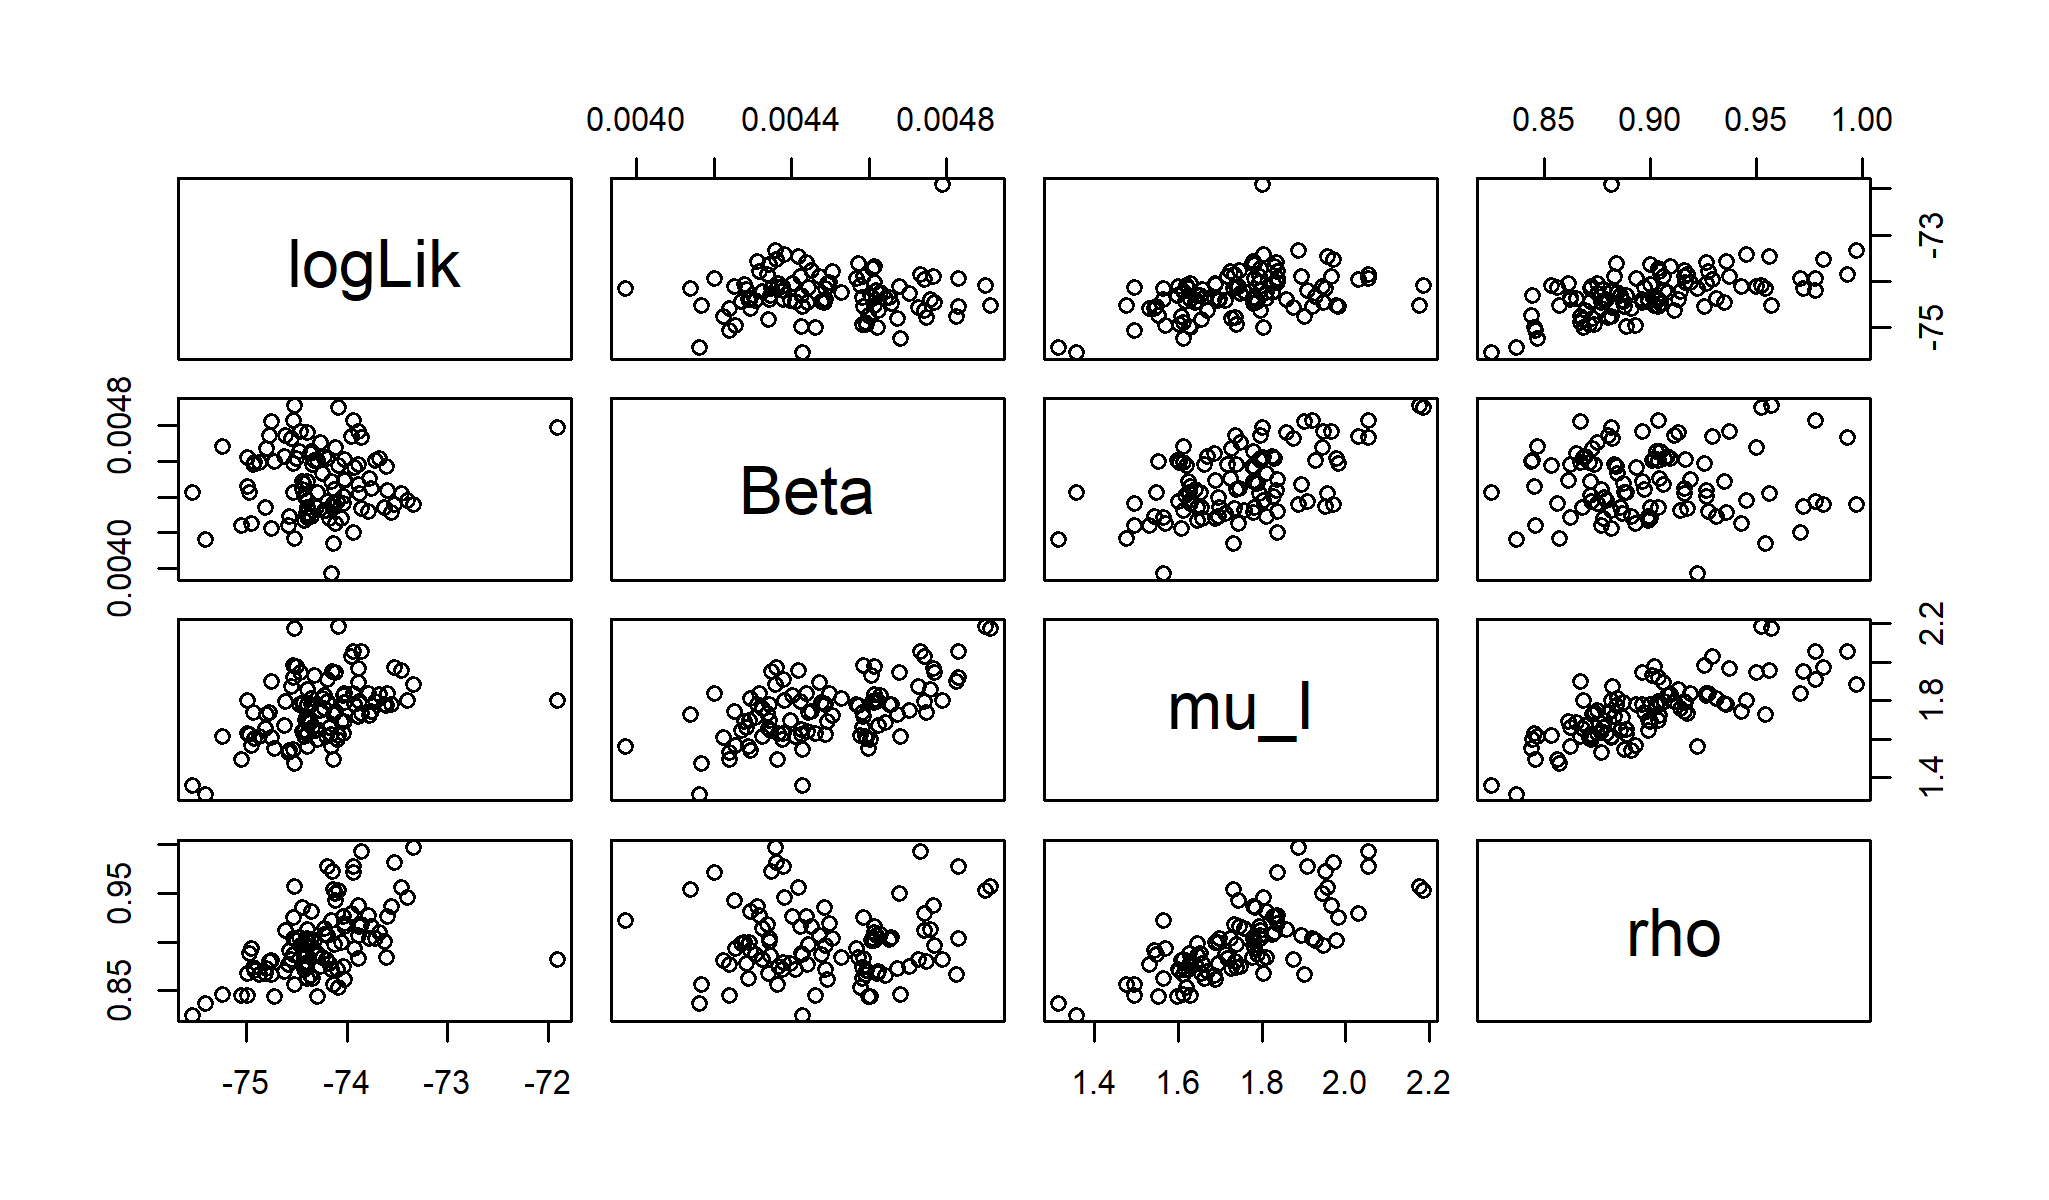
\includegraphics{figure/notes12-pairs_global-1} \end{center}

\begin{itemize}
\tightlist
\item
  We see that optimization attempts from diverse remote starting points
  end up with comparable likelihoods, even when the parameter values are
  quite distinct. This gives us some confidence in our maximization
  procedure.
\end{itemize}

\begin{center}\rule{0.5\linewidth}{\linethickness}\end{center}

\begin{center}\rule{0.5\linewidth}{\linethickness}\end{center}

\subsection{Diagnosing success or failure of the maximization
procedure}\label{diagnosing-success-or-failure-of-the-maximization-procedure}

\begin{itemize}
\item
  The \texttt{plot} method for an object of class \texttt{mif2d.pomp}
  presents some graphical convergence and filtering diagnostics for the
  maximization procedure.
\item
  It is often useful to look at superimposed convergence diagnostic
  plots for multiple Monte Carlo replications of the maximization
  procedure, perhaps with different starting values.
\item
  Concatenating objects of class \texttt{mif2d.pomp} gives a list of
  class \texttt{mif2List}. The \texttt{plot} method for a mif2List
  object gives us the superimposed convergence diagnostic plots.
\item
  Above, we built a list of mif2d.pomp objects for the global maximum
  likelihood search, fitting a model to the boarding school flu data.
  Let's first check the classes of the resulting objects.
\end{itemize}

\begin{Shaded}
\begin{Highlighting}[]
\KeywordTok{class}\NormalTok{(mifs_global)}
\end{Highlighting}
\end{Shaded}

\begin{verbatim}
## [1] "mif2List"
## attr(,"package")
## [1] "pomp"
\end{verbatim}

\begin{Shaded}
\begin{Highlighting}[]
\KeywordTok{class}\NormalTok{(mifs_global[[}\DecValTok{1}\NormalTok{]])}
\end{Highlighting}
\end{Shaded}

\begin{verbatim}
## [1] "mif2d.pomp"
## attr(,"package")
## [1] "pomp"
\end{verbatim}

\begin{Shaded}
\begin{Highlighting}[]
\KeywordTok{class}\NormalTok{(}\KeywordTok{c}\NormalTok{(mifs_global[[}\DecValTok{1}\NormalTok{]],mifs_global[[}\DecValTok{2}\NormalTok{]]))}
\end{Highlighting}
\end{Shaded}

\begin{verbatim}
## [1] "mif2List"
## attr(,"package")
## [1] "pomp"
\end{verbatim}

\begin{itemize}
\tightlist
\item
  Now, we can look at the diagnostics.
\end{itemize}

\subsubsection{Question: Interpret the
diagnostics}\label{question-interpret-the-diagnostics}

\begin{enumerate}
\def\labelenumi{\arabic{enumi}.}
\item
  Do these plots suggest we have successfully maximized the likelihood,
  or not? Why?
\item
  What would the convergence plots look like if we cooled too quickly?
  Or too slowly? Can you find evidence for either of these here? (The
  algorithmic parameter \texttt{cooling.fraction.50} is the fraction by
  which we decrease the random walk standard deviation in 50 filtering
  iterations.)
\item
  Here, we've done 300 mif iterations. Should we have done more? Could
  we have saved ourselves computational effort by doing less, without
  compromising our analysis?
\item
  Some parameter estimates show strong agreement between the different
  mif runs from different starting values. Others less so. How do you
  interpret this? Diversity in parameter estimates could be a signal of
  poor numerical maximization. It could signal a multi-modal likelhood
  surface. Or, it could simply correspond to a flat likelihood surface
  where the maximum is not precisely identifiable. Can we tell from the
  diagnostic plots which of these is going on here?
\item
  Maximization via particle filtering requires that the particle filter
  is working effectively. One way to monitor this is to pay attention to
  the
  \href{https://en.wikipedia.org/wiki/Effective_sample_size}{effective
  sample size} on the last filtering iteration. The effective sample
  size (ESS) is computed here as
  \[ \mathrm{ESS}_{n}= \frac{\left(\sum_{j=1}^J w_{n,j}\right)^2}{\sum_{j=1}^J w_{n,j}^2},\]
  where \(\{w_{n,j}\}\) are the weights defined in step 3 of the
  \protect\hyperlink{the-particle-filter}{particle filter}. The ESS
  approximates the number of independent, equally weighted, samples from
  the filtering distribution that would be equally informative to the
  one weighted sample that we have obtained by the particle filter. Do
  you have any concerns about the number of particles? 
\end{enumerate}

\begin{center}\rule{0.5\linewidth}{\linethickness}\end{center}

\begin{center}\rule{0.5\linewidth}{\linethickness}\end{center}

\subsection{Exercises}\label{exercises}

\subsubsection{Exercise: Construct a profile
likelihood}\label{exercise-construct-a-profile-likelihood}

\begin{itemize}
\item
  How strong is the evidence about the contact rate, \(\beta\), given
  this model and data? Use \texttt{mif2} to construct a profile
  likelihood. Due to time constraints, you may be able to compute only a
  preliminary version.
\item
  It is also possible to profile over the basic reproduction number,
  \(R_0=\beta P/\mu_I\). Is this more or less well determined that
  \(\beta\) for this model and data?
\end{itemize}

\begin{center}\rule{0.5\linewidth}{\linethickness}\end{center}

\begin{center}\rule{0.5\linewidth}{\linethickness}\end{center}

\subsubsection{Exercise: Check the model source
code}\label{exercise-check-the-model-source-code}

\begin{itemize}
\item
  Check the source code for the \texttt{bsflu} \texttt{pomp} object.
  Does the code implement the model described?
\item
  For various reasons, it can be surprisingly hard to make sure that the
  written equations and the code are perfectly matched. Here are some
  things to think about:
\end{itemize}

\begin{enumerate}
\def\labelenumi{\arabic{enumi}.}
\item
  Papers should be written to be readable to as broad a community as
  possible. Code must be written to run successfully. People do not want
  to clutter papers with numerical details which they hope and belief
  are scientifically irrelevant. What problems can arise due to this,
  and what solutions are available?
\item
  Suppose that there is an error in the coding of \texttt{rprocess}.
  Suppose that plug-and-play statistical methodology is used to infer
  parameters. A conscientious researcher carries out a simulation study,
  using \texttt{simulate} to generate some realizations from the fitted
  model and checking that the inference methodology can successfully
  recover the known parameters for this model, up to some statistical
  error. Will this procedure help to identify the error in
  \texttt{rprocess}? If not, how does one debug \texttt{rprocess}? What
  research practices help minimize the risk of errors in simulation
  code?
\end{enumerate}

\begin{center}\rule{0.5\linewidth}{\linethickness}\end{center}

\begin{center}\rule{0.5\linewidth}{\linethickness}\end{center}

\subsubsection{Exercise: Assessing and improving algorithmic
parameters}\label{exercise-assessing-and-improving-algorithmic-parameters}

Develop your own heuristics to try to improve the performance of
\texttt{mif2} in the previous example. Specifically, for a global
optimization procedure carried out using random starting values in the
specified box, let \(\hat\Theta_\mathrm{max}\) be a random Monte Carlo
estimate of the resulting MLE, and let \(\hat\theta\) be the true
(unknown) MLE. We can define the maximization error in the log
likelihood to be
\[e = \ell(\hat\theta) - E[\ell(\hat\Theta_\mathrm{max})].\] We cannot
directly evaluate \(e\), since there is also Monte Carlo error in our
evaluation of \(\ell(\theta)\), but we can compute it up to a known
precision. Plan some code to estimates \(e\) for a search procedure
using a computational effort of \(JM=2\times 10^7\), comparable to that
used for each mif computation in the global search. Discuss the
strengths and weaknesses of this quantification of optimization success.
See if you can choose \(J\) and \(M\) subject to this constraint,
together with choices of \texttt{rw.sd} and the cooling rate,
\texttt{cooling.fraction.50}, to arrive at a quantifiably better
procedure. Computationally, you may not be readily able to run your full
procedure, but you could run a quicker version of it.

\begin{center}\rule{0.5\linewidth}{\linethickness}\end{center}

\begin{center}\rule{0.5\linewidth}{\linethickness}\end{center}

\subsubsection{Exercise: Finding sharp peaks in the likelihood
surface}\label{exercise-finding-sharp-peaks-in-the-likelihood-surface}

\begin{itemize}
\tightlist
\item
  Even in this small, 3 parameter, example, it takes a considerable
  amount of computation to find the global maximum (with values of
  \(\beta\) around 0.004) starting from uniform draws in the specified
  box. The problem is that, on the scale on which ``uniform'' is
  defined, the peak around \(\beta\approx 0.004\) is very narrow.
  Propose and test a more favorable way to draw starting parameters for
  the global search, with better scale invariance properties.
\end{itemize}

\begin{center}\rule{0.5\linewidth}{\linethickness}\end{center}

\begin{center}\rule{0.5\linewidth}{\linethickness}\end{center}

\subsubsection{Exercise: Adding a latent
class}\label{exercise-adding-a-latent-class}

\begin{itemize}
\tightlist
\item
  Modify the model to include a latent period between becoming exposed
  and becoming infectious. See what effect this has on the maximized
  likelihood.
\end{itemize}

\begin{center}\rule{0.5\linewidth}{\linethickness}\end{center}

\begin{center}\rule{0.5\linewidth}{\linethickness}\end{center}

Acknowledgment

These notes draw on material developed for a short course on
\href{http://kingaa.github.io/sbied/}{Simulation-based Inference for
Epidemiological Dynamics} by Aaron King and Edward Ionides, taught at
the University of Washington Summer Institute in Statistics and Modeling
in Infectious Diseases, 2015.

\begin{center}\rule{0.5\linewidth}{\linethickness}\end{center}

\subsection*{References}\label{references}
\addcontentsline{toc}{subsection}{References}

\hypertarget{refs}{}
\hypertarget{ref-anonymous78}{}
Anonymous. 1978. Influenza in a boarding school. British Medical Journal
1:587.

\hypertarget{ref-arulampalam02}{}
Arulampalam, M. S., S. Maskell, N. Gordon, and T. Clapp. 2002. A
tutorial on particle filters for online nonlinear, non-Gaussian Bayesian
tracking. IEEE Trans. Sig. Proc. 50:174--188.

\hypertarget{ref-doucet01}{}
Doucet, A., N. de Freitas, and N. Gordon, editors. 2001. Sequential
Monte Carlo Methods in Practice. Springer-Verlag, New York.

\hypertarget{ref-ionides15}{}
Ionides, E. L., D. Nguyen, Y. Atchadé, S. Stoev, and A. A. King. 2015.
Inference for dynamic and latent variable models via iterated, perturbed
Bayes maps. Proceedings of the National Academy of Sciences of USA
112:719--724.

\hypertarget{ref-kitagawa87}{}
Kitagawa, G. 1987. Non-Gaussian state-space modeling of nonstationary
time series. Journal of the American Statistical Association
82:1032--1041.


\end{document}
